%\documentclass[a4paper,superscriptaddress,11pt]{quantumarticle}
%\documentclass[aps,twocolumn,longbibliography,english,superscriptaddress]{revtex4-1}
\documentclass{article}
\usepackage[preprint]{neurips_2020}
%\documentclass[a4paper,superscriptaddress,11pt]{article}
\pdfoutput=1
\usepackage[colorlinks=true,urlcolor=blue,citecolor=blue,linkcolor=blue]{hyperref}
\usepackage[english]{babel}
\usepackage[utf8]{inputenc}
\usepackage[T1]{fontenc}
\usepackage{amssymb}
\usepackage{tabularx}
\usepackage{upquote}
\usepackage{subcaption}
\usepackage{multicol}
%\usepackage{caption}
%\usepackage[plain]{algorithm}
\usepackage[ruled, vlined]{algorithm2e}
\usepackage{algpseudocode}
\usepackage{rotating}
%\usepackage{cite}
\usepackage{booktabs}
%\usepackage{unicode-math}
%\usepackage{algorithm}% http://ctan.org/pkg/algorithm
%\usepackage{algpseudocode}% http://ctan.org/pkg/algpseudocode
\usepackage{xcolor}% http://ctan.org/pkg/xcolor
\makeatletter
\newsavebox{\@brx}
\newcommand{\llangle}[1][]{\savebox{\@brx}{\(\m@th{#1\langle}\)}%
  \mathopen{\copy\@brx\kern-0.5\wd\@brx\usebox{\@brx}}}
\newcommand{\rrangle}[1][]{\savebox{\@brx}{\(\m@th{#1\rangle}\)}%
  \mathclose{\copy\@brx\kern-0.5\wd\@brx\usebox{\@brx}}}
\makeatother
\usepackage{bbm}
\usepackage{jlcode}
\usepackage{graphicx}
\usepackage{amsmath,color,amsthm}
\usepackage{mathrsfs}
\usepackage{float}
\usepackage[normalem]{ulem}
\usepackage{indentfirst}
\usepackage{txfonts}
\usepackage[epsilon, tsrm, altpo]{backnaur}

\newcolumntype{b}{X}
\newcolumntype{s}{>{\hsize=.7\hsize}X}
\usepackage{listings}
\lstset{
    language=Julia,
    basicstyle=\ttfamily\scriptsize,
    numberstyle=\scriptsize,
    % numbers=left,
    backgroundcolor=\color{gray!7},
    %backgroundcolor=\color{white},
    %frame=single,
    xleftmargin=2em,
    tabsize=2,
    rulecolor=\color{black!15},
    %title=\lstname,
    %escapeinside={\%(*}{*)},
    breaklines=true,
    %breakatwhitespace=true,
    %framextopmargin=2pt,
    %framexbottommargin=2pt,
    frame=bt,
    extendedchars=true,
    inputencoding=utf8,
    columns=fullflexible,
}

\tolerance=1
\emergencystretch=\maxdimen
\hyphenpenalty=1000
\hbadness=1000

\makeatletter

%%%%%%%%%%%%%%%%%%%%%%%%%%%%%% User specified LaTeX commands.

%Journal reference.  Comma sets off: name, vol, page, year
\def\journal #1, #2, #3, 1#4#5#6{{\sl #1~}{\bf #2}, #3 (1#4#5#6) }
\def\pr{\journal Phys. Rev., }
\def\prb{\journal Phys. Rev. B, }
\def\prl{\journal Phys. Rev. Lett., }
\def\pl{\journal Phys. Lett., }
%\def\np{\journal Nucl. Phys., }


%%%%%%%%%%%%%%%%%%%%%%%%%%%%%%%%%%%%%%%%%%%%%%%%%%%%%%%%%%%%%%%%%%%%%%%%%%%%%%%%%%%%%%%%%%%%%%%%%%%%%%%%%%%%%%%%%%%%%%%%%%%%%%%%%%%%%%%%%%%%%%%%%%%%%%%%%%%%%%%%%%%%%%%%%%%%%%%%%%%%%%%%%%%%%%%%%%%%%%%%%%%%%%%%%%%%%%%%%%%%%%%%%%%%%%%%%%%%%%%%%%%%%%%%%%%%


%\usepackage{CJK}
%\usepackage[colorlinks, citecolor=blue]{hyperref}
\DeclareMathOperator*{\argmax}{arg\,max}

%%%%%% Shortcut related
\newcommand{\<}{\langle}
\renewcommand{\>}{\rangle}
\newcommand{\out}{{\vx^L}}
\newcommand{\inp}{{\vx^0}}
\newcommand{\cquad}{{{ }_{\quad}}}
\newcommand{\pluseq}{\mathrel{+}=}
\newcommand{\minuseq}{\mathrel{-}=}
\newcommand{\vx}{{\mathbf{x}}}
\newcommand{\vg}{{\mathbf{g}}}
\newcommand{\vp}{{\mathbf{p}}}
\newcommand{\vy}{{\mathbf{y}}}
\newcommand{\Var}{{\mathrm{Var}}}
\newcommand{\Mean}{{\mathrm{E}}}
\newcommand{\vvalue}{{\texttt{value}}}
\newcommand{\grad}{{\texttt{grad}}}
\newcommand{\parameter}{{\texttt{parameter}}}
%%%%%% Convention related
\newcommand{\SWAP}{{\rm SWAP}}
\newcommand{\CNOT}{{\rm CNOT}}
\newcommand{\X}{{\rm X}}
\renewcommand{\H}{{\rm H}}
\newcommand{\Rx}{{\rm Rx}}
\renewcommand{\v}[1]{{\bf #1}}
\newcommand{\dataset}{{\mathcal{D}}}
\newcommand{\wfunc}{{\psi}}
\newcommand{\SU}{{\rm SU}}
\newcommand{\UU}{{\rm U}}
\newcommand{\thetav}{{\boldsymbol{\theta}}}
\newcommand{\gammav}{{\boldsymbol{\gamma}}}
\newcommand{\thetai}{{\theta^\alpha_l}}
\newcommand{\Expect}{{\mathbb{E}}}
\newcommand{\Tr}{{\rm Tr}}
\newcommand{\etc}{{\it etc~}}
\newcommand{\etal}{{\it etal~}}
\newcommand{\xset}{\mathbf{X}}
\newcommand{\fl}{\texttt{fl}}
\newcommand{\pdata}{\mathbf{\pi}}
\newcommand{\q}{\mathbf{q}}
\newcommand{\epdata}{\mathbf{\hat{\pi}}}
\newcommand{\gammaset}{\boldsymbol{\Gamma}}
\newcommand{\ei}{{\mathbf{e}_l^\alpha}}
\newcommand{\vtheta}{{\boldsymbol{\theta}}}
\newcommand{\sigmag}{{\nu}}
\newcommand{\sigmai}[2]{{\sigma^{#2}_{#1}}}
\newcommand{\qi}[1]{{q^{\alpha_{#1}}_{#1}}}
\newcommand{\BAS}{Bars-and-Stripes}
\newcommand{\circled}[1]{\raisebox{.5pt}{\textcircled{\raisebox{-.9pt} {#1}}}}

\newcommand{\qexpect}[1]{{\left\langle #1\right\rangle}}
\newcommand{\expect}[2]{{\mathop{\mathbb{E}}\limits_{\substack{#2}}\left[#1\right]}}
\newcommand{\var}[2]{{\mathop{\mathrm{Var}}\limits_{\substack{#2}}\left(#1\right)}}
\newcommand{\pshift}[1]{{p_{\thetav+#1}}}
\newcommand{\upcite}[1]{\textsuperscript{\cite{#1}}}
\newcommand{\Eq}[1]{Eq.~(\ref{#1})}
\newcommand{\Fig}[1]{Fig.~\ref{#1}}
\newcommand{\Lst}[1]{Listing.~\ref{#1}}
\newcommand{\Ref}[1]{Ref.~\cite{#1}}
\newcommand{\Tbl}[1]{Table~\ref{#1}}
\newcommand{\Sec}[1]{Sec.~\ref{#1}}
\newcommand{\App}[1]{Appendix \ref{#1}}
\newcommand{\bra}[1]{\mbox{$\left\langle #1 \right|$}}
\newcommand{\ket}[1]{\mbox{$\left| #1 \right\rangle$}}
\newcommand{\braket}[2]{\mbox{$\left\langle #1 | #2 \right\rangle$}}
\newcommand{\tr}[1]{\mathrm{tr}\mbox{$\left[ #1\right]$}}

\newcommand{\ra}[1]{\renewcommand{\arraystretch}{#1}}

%%%%%% Comment related
\newcommand{\red}[1]{[{\bf  \color{red}{LW: #1}}]}
\newcommand{\xred}[1]{[{\bf  \color{red}{\sout{LW: #1}}}]}
\newcommand{\blue}[1]{[{\bf  \color{blue}{JG: #1}}]}
\newcommand{\violet}[1]{[{\bf  \color{violet}{MLS: #1}}]}
\newcommand{\green}[1]{[{\bf  \color{green}{TZ: #1}}]}
\newcommand{\xgreen}[1]{[{\bf  \color{green}{\sout{TZ: #1}}}]}
\newcommand{\xblue}[1]{[{\bf  \color{blue}{\sout{JG: #1}}}]}
\newcommand{\material}[1]{\iffalse[{\bf  \color{cyan}{Material: #1}}]\fi}
\newcommand{\orange}[1]{\iffalse[{\bf  \color{orange}{Jo: #1}}]\fi}

\newtheorem{theorem}{\textit{Theorem}}
\theoremstyle{definition}\newtheorem{definition}{\textit{Definition}}

\makeatother

\begin{document}
\title{Differentiate Everything with a Reversible Domain-Specific Language}

\author{Jin-Guo Liu\\
Institute of Physics, Chinese Academy of Sciences,\\Beijing 100190, China\\
\texttt{cacate0129@iphy.ac.cn}\\
\And
Taine Zhao\\
Department of Computer Science, University of Tsukuba\\
\texttt{thaut@logic.cs.tsukuba.ac.jp}\\
}
%\author{Lei Wang}
%\email{wanglei@iphy.ac.cn}
%\affiliation{Institute of Physics, Chinese Academy of Sciences, Beijing 100190, China}
%\affiliation{CAS Center for Excellence in Topological Quantum Computation, University of Chinese Academy of Sciences, Beijing 100190, China}
%\affiliation{Songshan Lake Materials Laboratory, Dongguan, Guangdong 523808, China}

%\author{Jin-Guo Liu}
%\email{cacate0129@iphy.ac.cn}
%\affiliation{Institute of Physics, Chinese Academy of Sciences, Beijing 100190, China}

%\author{Taine Zhao}
%\affiliation{Department of Computer Science, University of Tsukuba}

\maketitle

\begin{abstract}
Traditional machine instruction level reverse-mode automatic differentiation (AD) suffers from the problem of having a space overhead that linear to time in order to trace back the computational state, which is also the source of poor performance. In reversible programming, a program can be executed bi-directionally, which means we do not need any additional design to trace back the computational state. This paper answers how practical it is to implement a machine-instruction level reverse mode AD in a reversible programming language. By implementing sparse matrix operations and some machine learning applications in our reversible eDSL NiLang, and benchmark the performance with state-of-the-art AD frameworks, our answer is a definite positive.
NiLang is an open-source r-Turing complete reversible eDSL in Julia. It empowers users the flexibility to tradeoff time, space, and energy rather than caching data into a global tape. Manageable memory allocation makes it an excellent tool to differentiate GPU kernels too.
\end{abstract}

%\begin{multicols}{2}
\section{Introduction}\label{sec:intro}
    Computing the gradients of a numeric model $f : \mathbb{R}^m \rightarrow \mathbb{R}^n$ plays a crucial role in scientific computing. Consider a computing process
\begin{align*}
    &\vx^1 = f_1(\vx^0)\\
    &\vx^2 = f_2(\vx^1)\\
    &\ldots\\
    &\vx^L = f_L(\vx^{L-1})
\end{align*}
where $x^0\in R^m$, $x^L\in R^n$, $L$ is the depth of computing.
The Jacobian of this program is a $n\times m$ matrix $J_{ij} \equiv \frac{\partial x^L_i}{\partial x_j^0}$, where $x_j^0$ and $x_i^L$ are single elements from inputs and outputs.
Computing the Jacobian or part of the Jacobian automatically is what we called automatic differentiation (AD). It can be classified into three classes, the forward mode AD, the backward mode AD and the mixed mode AD~\cite{Hascoet2013}.
    The forward mode AD computes the Jacobian matrix elements related to a single input using the chain rule $\frac{\partial \vx^k}{\partial x^0_j} = \frac{\partial \vx^k}{\partial \vx^{k-1}}\frac{\partial \vx^{k-1}}{\partial x^0_j}$ with $j$ the column index, while a backward mode AD computes Jacobian matrix elements related to a single output using the chain rule in the reverse direction $\frac{\partial \vx^L_i}{\partial x^{k-1}} = \frac{\partial \vx^L_i}{\partial \vx^{k}}\frac{\partial \vx^{k}}{\partial x^{k-1}}$ with $i$ the row index.
    In variational applications where the loss function always outputs a scalar, the backward mode AD is preferred.
However, implementing backward mode AD is harder than implementing its forward mode counterpart, because it requires propagating the gradients in the inverse direction of computing the loss. The backpropagation of gradients requires
\begin{enumerate}
    \item an approach to trace back the computational process,
    \item caching variables required for computing gradients.
\end{enumerate}
    %The computational process is often represented as a computational graph, a directed acyclic graph (DAG) representing the relationship between data and functions. Comparing with a general computer program, a computational graph does not have mutable variables and control flows.
    Most popular AD packages in the market implements the computational graph to solve above issues at the tensor level.
    In Pytorch~\cite{Paszke2017} and Flux~\cite{Innes2018a}, every variable has a tracker field. When applying a predefined primitive function on a variable, the variable's tracker field keeps track of this function as well as data needed in backpropagation.
    TensorFlow~\cite{Tensorflow2015} also implements the computational graph, but it builds a static computational graph as a description of the program before actual computation happens.
    %These packages all prefer tensor types, where the overhead of memory allocations is less significant.
    These frameworks sometimes fail to meet the diverse needs in research, for example, in physics research,
    \begin{enumerate}
        \item People need to differentiate over sparse matrix operations that are important for Hamiltonian engineering~\cite{Xie2020}, like solving dominant eigenvalues and eigenvectors~\cite{Golub2012},
        \item People need to backpropagate singular value decomposition (SVD) function and QR decomposition in tensor network algorithms to study the phase transition problem~\cite{Golub2012,Liao2019,Seeger2017,Wan2019,Hubig2019,Wan2019},
        \item People need to differentiate over a quantum simulation where each quantum gate is an inplace function that changes the quantum register directly~\cite{Luo2019}.
    \end{enumerate}
    %Scientists have put lots of effort to derive new backward rules for these needs.

    To solve these issues better, we need a hardware instruction level AD. Source code transformation based AD packages like Tapenade~\cite{Hascoet2013} and Zygote~\cite{Innes2018, Innes2019} are closer to this goal. They read the source code from a user and generate a new code that computes the gradients for users. However, these packages have their own limitations too. In many practical applications, an elementary level differentiable program that might do billions of computations will cache intermediate results to a global storage. Frequent caching of data slows down the program significantly, and the memory usage will become a bottleneck as well. With these AD tools, it is still nearly impossible to automatically generate the backward rules for BLAS functions and sparse matrix operations with a performance comparable to the state-of-the-art.% A better solution to memory management must be found to make source-to-source AD practical.

    We propose to implement hardware instruction level AD on a reversible (domain-specific) programming language~\cite{Perumalla2013,Frank2017}. So that the intermediate states of a program can be traced backward with no extra effort. The overhead of reverse mode AD becomes the overhead of reversing a program, where the later has the advantage of efficient and controllable memory management. There have been many prototypes of reversible languages like Janus~\cite{Lutz1986}, R (not the popular one)~\cite{Frank1997}, Erlang~\cite{Lanese2018} and object-oriented ROOPL~\cite{Haulund2017}. % These languages have reversible control flow that allows users to input an additional postcondition in control flows to help programs run backward.
    In the past, the primary motivation of studying reversible programming is to support reversible computing devices~\cite{Frank1999} like adiabatic complementary metal–oxide–semiconductor (CMOS)~\cite{Koller1992}, molecular mechanical computing system~\cite{Merkle2018} and superconducting system~\cite{Likharev1977,Semenov2003}, where a reversible computing device is more energy-efficient from the perspective of information and entropy, or by the Landauer's principle~\cite{Landauer1961}.
    After decades of efforts, reversible computing devices are very close to providing productivity now. As an example, adiabatic CMOS can be a better choice in a spacecraft~\cite{Hanninen2014, Debenedictis2017}, where energy is more valuable than device itself.
    Reversible programming is interesting to software engineers too, because it is a powerful tool to schedule asynchronious events~\cite{Jefferson1985} and debug a program bidirectionally~\cite{Boothe2000}.
    However, the field of reversible computing faces the issue of having not enough funding in recent decade~\cite{Frank2017}. As a result, not many people studying AD know the marvelous designs in reversible computing. People have not connected it with automatic differentiation seriously, even though they have many similarities. This paper aims to break the information barrier between the machine learning community and the reversible programming community in our work and provide yet another strong motivation to develop reversible programming.

    In this paper, we first introduce the language design of a reversible programming language and introduce our reversible eDSL NiLang in \Sec{sec:lang}.
    In \Sec{sec:bp}, we explain the implementation of automatic differentiation in this eDSL.
    In \Sec{sec:example}, we show several examples.
    In \Sec{sec:benchmark}, we benchmark the performance of NiLang with other AD packages and explain why reversible programming AD is fast.
    In \Sec{sec:discussion}, we discuss several important issues, the time-space  tradeoff, reversible instructions and hardware, and finally, an outlook to some open problems to be solved.
    In the appendix, we show the grammar of NiLang and other technical details.


\section{Language design}\label{sec:lang}

    \subsection{Introductions to reversible language design}
    In a modern programming language, functions are pushed to a global stack for scheduling. The memory layout of a function consists of input arguments, a function frame with information like the return address and saved memory segments, local variables, and working stack. After the call, the function clears run-time information, only stores the return value. In reversible programming, this kind of design is no longer the best practice. One can not discard input variables and local variables easily after a function call, since discarding information may ruin reversibility. For this reason, reversible functions are very different from irreversible ones from multiple perspectives.

\subsubsection{Memory management}
    A distinct feature of reversible memory management is, the content of a variable must be known when it is deallocated.
    We denote the allocation of a zero emptied memory as \texttt{x $\leftarrow$ 0}, and the corresponding deallocation as \texttt{x $\rightarrow$ 0}.
    A variable $x$ can be allocated and deallocated in a local scope, which is called an ancilla.
    It can also be pushed to a stack and used later with a pop statement.
    This stack is similar to a traditional stack, except it zero-clears the variable after pushing and presupposes that the variable being zero-cleared before popping.
\begin{figure}
    \centerline{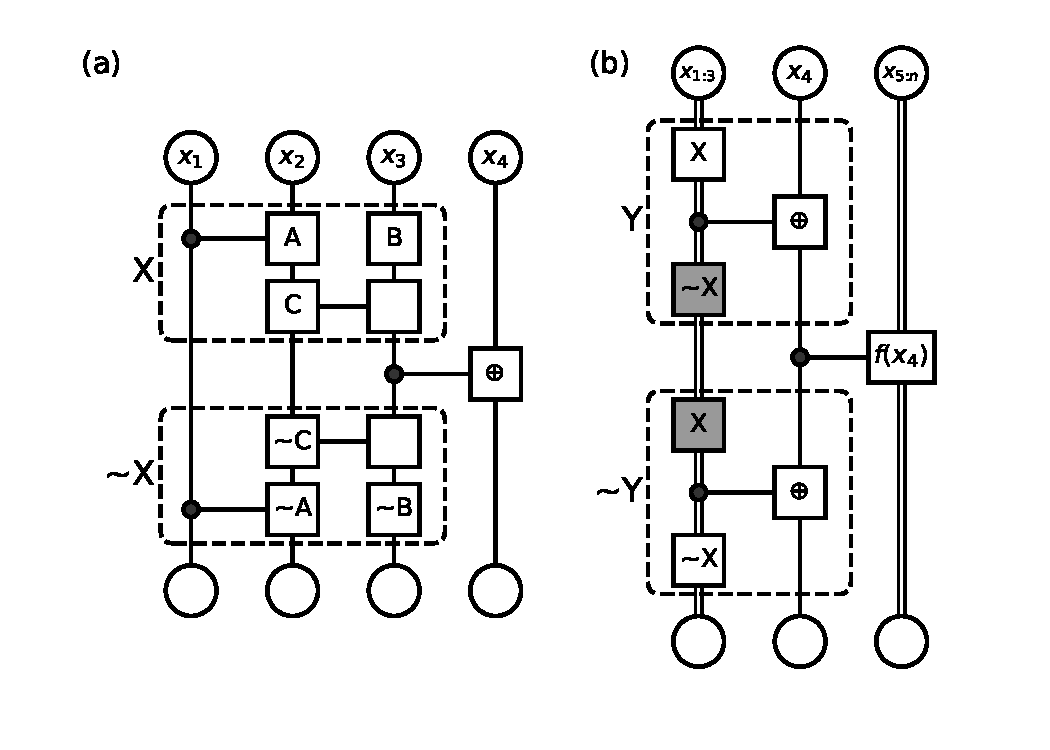
\includegraphics[width=0.6\columnwidth,trim={0 1cm 0 0cm},clip]{fig6.pdf}}
    \caption{Two computational processes represented in memory oriented computational graph, where (a) is a subprogram in (b). In these graphs, a vertical single line represents one variable, a vertical double line represents multiple variables, and a parallel line represents a function. A dot at the cross represents a control parameter of a function and a box at the cross represents a mutable parameter of a function.
    }\label{fig:ccu}
\end{figure}

Knowing the contents in the memory when deallocating is not easy. Hence Charles H. Bennett introduced the famous compute-copy-uncompute paradigm~\cite{Bennett1973} for reversible programming.
To explain how it works, we introduce the memory oriented computational graph, as shown in \Fig{fig:ccu}.
Notations are highly inspired by the quantum circuit representation. A vertical line is a variable and a horizontal line is a function. When a variable is used by a function, depending on whether its value is changed or not, we put a box or a dot at the line cross. It is different from the computational graph for being a hypergraph rather than a simple graph, because a variable can be used by multiple functions now.
In panel (a). The subprogram in dashed box \texttt{X} is executed on space $x_{1\colon3}$ represents the computing stage. In the copying stage, the content in $x_3$ is read out to a pre-emptied memory $x_4$ through inplace add \texttt{+=}. Since this copy operation does not change contents of $x_{1\colon3}$, we can use the uncomputing operation \texttt{$\sim$X} to undo all the changes to these registers. Now we computing the result $x_4$ without modifying the contents in $x_{1\colon3}$. If any of them is in a known state, it can be deallocated immediately.
In panel (b), we can use the subprogram defined in (a) maked as Y to generate $x_{5\colon n}$ without modifying the contents of variables $x_{1\colon 4}$.
It is easy to see that although this uncompute-copy-uncompute design pattern can restore memories to known state, it has computational overhead.
Both $X$ and $\sim X$ are executed twice in the program (b), which is not necessary. We can cancel a pair of $X$ and $\sim X$ (the gray boxes). By doing this, we are not allowed to deallocate the memory $x_{1\colon3}$ during computing $f(x_{5\colon n})$. This is the famous time-space tradeoff that playing the central role in reversible programming. The tradeoff strategy will be discussed in detail in \Sec{sec:timespace}.

\subsubsection{Control flows}
One can define reversible \texttt{if}, \texttt{for} and \texttt{while} statements in a slightly different way comparing with its irreversible counterpart. The reversible \texttt{if} statement is shown in \Fig{fig:controlflow} (a). Its condition statement contains two parts, a precondition and a postcondition. The precondition decides which branch to enter in the forward execution, while the postcondition decides which branch to enter in the backward execution. After executing the specific branch, the program checks the consistency between precondition and postcondition to make sure they are consistent.
The reversible \texttt{while} statement in \Fig{fig:controlflow} (b) also has two condition fields. Before executing the condition expressions, the program preassumes the postcondition is false.
After each iteration, the program asserts the postcondition to be true. In the reverse pass, we exchange the precondition and postcondition.
The reversible \texttt{for} statement is similar to irreversible ones except that after executing the loop, the program checks the values of these variables to make sure they are not changed. In the reverse pass, we exchange \texttt{start} and \texttt{stop} and inverse the sign of \texttt{step}.
\begin{figure}
    \centerline{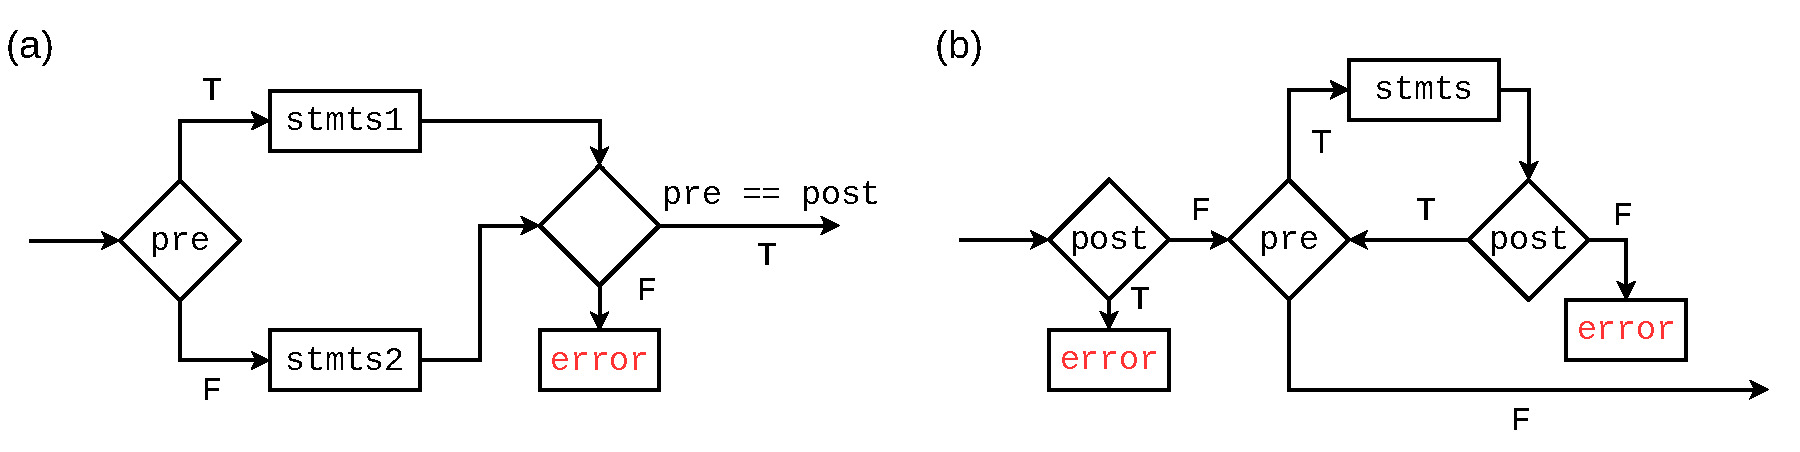
\includegraphics[width=0.9\columnwidth,trim={0 0cm 0 0cm},clip]{controlflow_v2.pdf}}
    \caption{The flow chart for reversible (a) \texttt{if} statement and (b) \texttt{while} statement. ``pre'' and ``post'' represents precondition and postconditions respectively.}\label{fig:controlflow}
\end{figure}

\subsubsection{Arithmetic instructions}
Every arithmetic instruction has a unique inverse that can undo the changes.
\begin{itemize}
    \item For logical operations, \texttt{y $\veebar$= f(args...)} is self reversible.
    \item For integer and floating point arithmetic operations, we treat \texttt{y += f(args...)} and \texttt{y -= f(args...)} as reversible to each other. Here \texttt{f} can be an arbitrary pure function such as \texttt{identity}, \texttt{*}, \texttt{/} and \texttt{\^}. Let's forget the floating point rounding errors for the moment and discuss in detail in \Sec{sec:hardware}.
    \item For logartihmic number and tropical number algebra~\cite{Speyer2009}, \texttt{y *= f(args...)} and \texttt{y /= f(args...)} as reversible to each other. Notice the zero element ($-\infty$) in the Tropical algebra is not considered here.
\end{itemize}
Besides the above two types of operations, \texttt{SWAP} operation that exchanges the contents in two memory spaces is also widely used in reversible computing systems.

\subsection{Differetiable Reversible eDSL: NiLang}
    We develop an embedded domain-specific language (eDSL) NiLang in Julia language~\cite{Bezanson2012,Bezanson2017} that implements reversible programming. One can write reversible control flows, instructions, and memory managements inside this macro.
Julia is a popular language for scientific programming. We choose Julia as the host language for multiple purposes. The most important consideration is speed that crucial for a machine instruction level AD. Its clever design of type inference and just in time compiling provides a C like speed.
Also, it has a rich ecosystem for meta-programming. The package for pattern matching \href{https://github.com/thautwarm/MLStyle.jl}{MLStyle} allow us to define an eDSL conveniently. Last but not least, its multiple-dispatch provides the polymorphism that will be used in our AD engine.
%In the past, we see many implementations of AD languages work as an independent language.
%However, we hope our eDSL can benefit people in Julia's community directly.
The main feature of NiLang is contained in a single macro \texttt{@i} that compiles a reversible function.
The allowed statements in this eDSL are shown in \App{app:grammar}.
We can use \texttt{macroexpand} to show the compiling a reversible function to the native Julia function.

\begin{minipage}{.88\columnwidth}
\begin{lstlisting}
julia> using NiLangCore, MacroTools

julia> MacroTools.prettify(@macroexpand @i function f(x, y)
           SWAP(x, y)
       end)
quote
    $(Expr(:meta, :doc))
    function $(Expr(:where, :(f(x, y))))
        dove = wrap_tuple(SWAP(x, y))
        x = dove[1]
        y = dove[2]
        (x, y)
    end
    if NiLangCore._typeof(f) != _typeof(~f)
        function $(Expr(:where, :((hummingbird::_typeof(~f))(x, y))))
            toad = wrap_tuple((~SWAP)(x, y))
            x = toad[1]
            y = toad[2]
            (x, y)
        end
    end
end
\end{lstlisting}
\end{minipage}

Here, the version of NiLang is v0.4.0.
Macro \texttt{@i} generates two functions that reversible to each other \texttt{f} and \texttt{$\sim$f}. \texttt{$\sim$f} is an callable of type \texttt{Inv\{typeof(f)\}}, where the type parameter \texttt{typeof(f)} stands for the type of the function \texttt{f}.
In the body of \texttt{f}, \texttt{NiLangCore.wrap\_tuple} is used to unify output data types to tuples.
The outputs of \texttt{SWAP} are assigned back to its input variables.
At the end of this function, this macro attaches a return statement that returns all input variables.

The compilation of a reversible function to native Julia functions is consisted of three stages: \textit{preprocessing}, \textit{reversing} and \textit{translation}.
\Fig{fig:compiling} shows the compilation of the complex valued log function body, which is originally defined as follows.

\begin{minipage}{.88\columnwidth}
\begin{lstlisting}[mathescape=true,caption={Reversible implementation of the complex valued log function.},label={lst:complex}]
@i function (:+=)(log)(y!::Complex{T}, x::Complex{T}) where T
    @routine begin
        n ← zero(T)
        n += abs(x)
    end
    y!.re += log(n)
    y!.im += angle(x)
    ~@routine
end
\end{lstlisting}
\end{minipage}

\begin{figure}
    \centerline{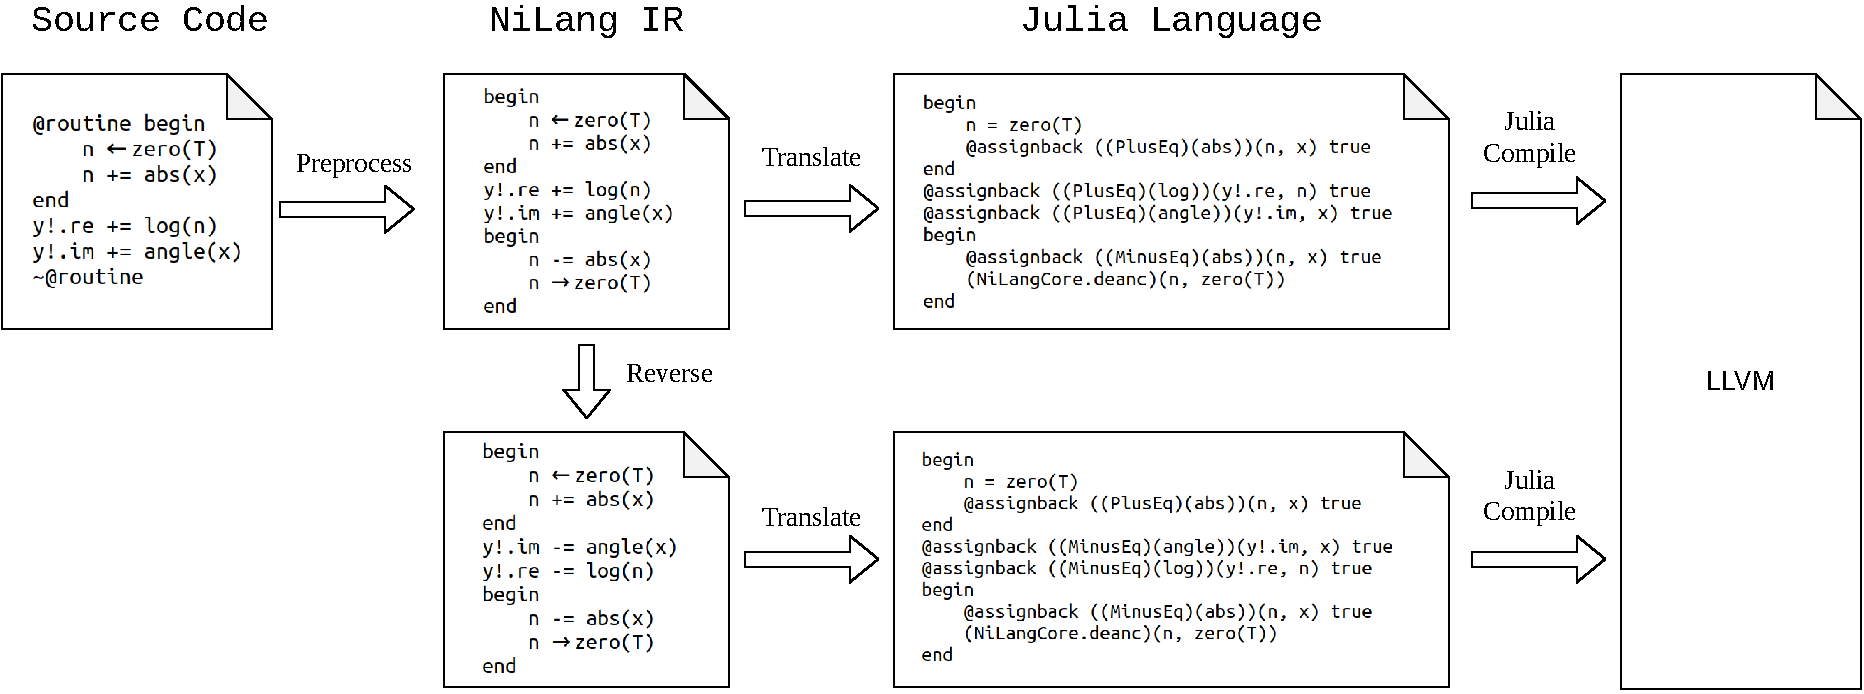
\includegraphics[width=0.95\columnwidth,trim={0cm 0cm 0cm 0cm},clip]{compiling_v2.pdf}}
    \caption{Compiling the body of the complex valued log function defined in \Lst{lst:complex}.}\label{fig:compiling}
\end{figure}

In the \textit{preprocessing} stage, the compiler pre-processes human inputs to reversible NiLang IR.
The preprocessor removes redundant grammars and expands shortcuts. In the left most code box in \Fig{fig:compiling}, one uses \texttt{@routine <stmt>} statement to record a statement, and \texttt{$\sim$@routine} to insert the corresponding inverse statement for uncomputing.
The computing-uncomputing macros \texttt{@routine} and \texttt{$\sim$@routine} is expanded in this stage.
Here, one can input ``$\leftarrow$'' and ``$\rightarrow$'' by typing ``$\backslash$leftarrow[TAB KEY]'' and ``$\backslash$rightarrow[TAB KEY]'' respectively in a Julia editor or REPL.

In the \textit{reversing} stage, based on this symmetric and reversible IR, the compiler generates reversed statements according to table \Tbl{tbl:revstatements}.

\begin{table}[h!]\centering
    \footnotesize
\begin{minipage}{\columnwidth}
\ra{1.3}
    \scalebox{1.0}{
        \begin{tabularx}{\textwidth}{X X X}\toprule
            \textbf{Statement} & \textbf{Meaning} & \textbf{Inverse}\\
            \hline
            \texttt{<f>(<args>...)} & function call & \texttt{($\sim$<f>)(<args>...)}\\
            \hline
            \texttt{<f>.(<args>...)} & broadcast a function call & \texttt{<f>.(<args>...)}\\
            \hline
            \texttt{<y> += <f>(<args>...)} & inplace add instruction & \texttt{<y> -= <f>(<args>...)}\\
            \hline
            \texttt{<y> $\veebar$= <f>(<args>...)} & inplace XOR instruction & \texttt{<y> $\veebar$= <f>(<args>...)}\\
            \hline
            \texttt{<a> $\leftarrow$ <expr>} & allocate a new variable & \texttt{<a> $\rightarrow$ <expr>}\\
            \hline
            \texttt{begin}\newline \texttt{$\cquad$<stmts>}\newline \texttt{end} & statement block & \texttt{begin}\newline \texttt{$\cquad$ $\sim$(<stmts>)}\newline \texttt{end}\\
            \hline
            \texttt{if (<pre>, <post>)}\linebreak \texttt{$\cquad$<stmts1>}\newline \texttt{else}\newline \texttt{$\cquad$<stmts2>}\newline \texttt{end} & if statement & \texttt{if (<post>, <pre>)}\newline \texttt{$\cquad$$\sim$(<stmts1>)}\newline \texttt{else}\newline \texttt{$\cquad$ $\sim$(<stmts2>)}\newline \texttt{end}\\ %$
            \hline
            \texttt{while (<pre>, <post>)}\newline \texttt{$\cquad$<stmts>} \newline \texttt{end} & while statement & \texttt{while (<post>, <pre>)}\newline $\cquad$  \texttt{$\sim$(<stmts>)}\newline \texttt{end}\\
            \hline
            \texttt{for <i>=<m>:<s>:<n>}\newline $\cquad$\texttt{<stmts>}\newline \texttt{end} & for statement & \texttt{for <i>=<m>:-<s>:<n>}\newline $\cquad$ \texttt{$\sim$(<stmts>)}\newline \texttt{end}\\
            \bottomrule
        \end{tabularx}
    }
    \caption{Basic statements in NiLang IR.
    ``$\sim$'' is the symbol for reversing a statement or a function.
    ``.'' is the symbol for the broadcasting magic in Julia,
    \texttt{<pre>} stands for precondition, and \texttt{<post>} stands for postcondition
``\texttt{begin <stmts> end}'' is the code block statement in Julia.
It can be inverted by reversing the order as well as each element in it.
}\label{tbl:revstatements}
\end{minipage}
\end{table}

In the \textit{translation} stage, the compiler translates this reversible IR as well as its inverse to native Julia code. It adds \texttt{@assignback} before each function call, inserts codes for reversibility check, and handle control flows.
We can expand the \texttt{@assignback} macro to see the compiled expression.

\begin{minipage}{.88\columnwidth}
\begin{lstlisting}
julia> macroexpand(Main, :(@assignback PlusEq(log)(y!.re, n)))
quote
    var"##277" = (PlusEq(log))(y!.re, n)
    begin
        y! = chfield(y!, Val{:re}(), ((NiLangCore.wrap_tuple)(var"##277"))[1])
        n = ((NiLangCore.wrap_tuple)(var"##277"))[2]
    end
end
\end{lstlisting}
\end{minipage}

Here, the function \texttt{chfield} returns a complex number with an updated \texttt{re} field. This updated value is then assigned back to \texttt{y!}.
In other words, this macro simulates ``inplace'' operations on immutable types.
Except immutable fields, mappings and indexing can also be modified. We call an expression that directly modifiable in NiLang a \textit{dataview}, it can be a variable itself, a field or an element of a dataview, or a bijective mapping of a dataview.
The following are some examples of dataviews

\begin{multicols}{2}
\begin{list}{$\circ$}{}
\item real(x)
\item x.re
\item x[3]
\item x\textquotesingle
\item real.(x)
\item (x, y, z)
\item tget(x, 2)  \# tuple get index
\item -x[2].re\textquotesingle
\end{list}
\end{multicols}

%One can skip the assign back operation by inserting \texttt{@skip!} macro before a variable like \texttt{f(y, @skip! x)} to avoid automatic assigning back.

As a final step, the compiler attaches a return statement that returns all updated input arguments at the end of a function definition.
Now, the function is ready to execute on the host language.
One can also define a reversible constructor and destructor, we put this part in \App{app:constructor}.

\section{Reversible automatic differentiation}\label{sec:bp}

\subsection{First order gradient}\label{sec:jacobian}
\begin{figure}
    \centerline{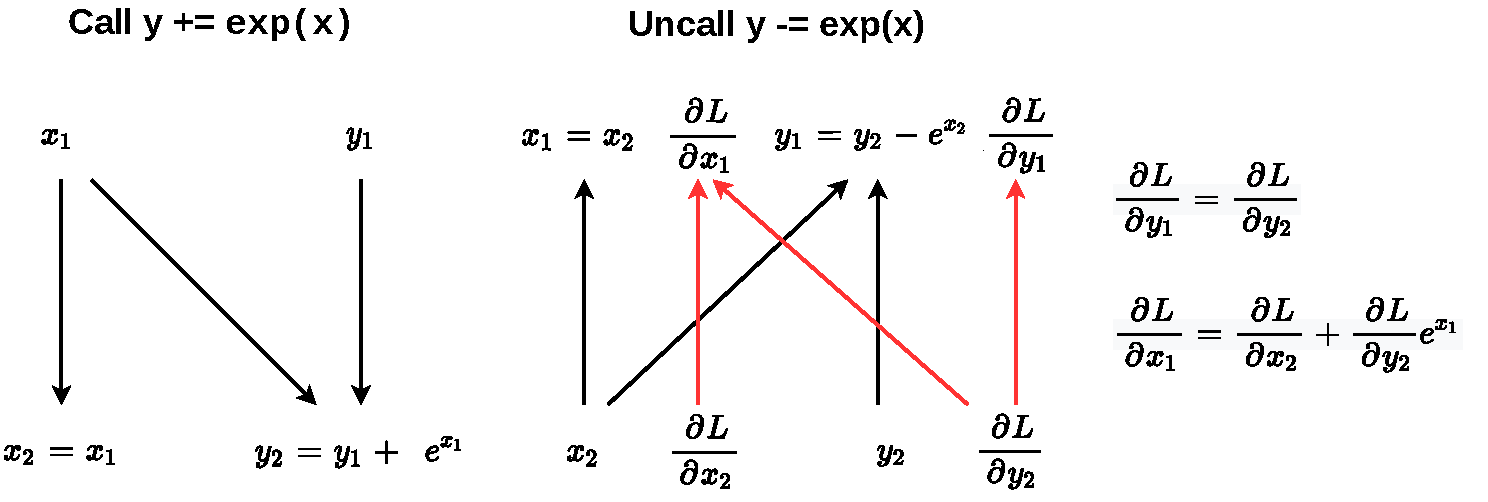
\includegraphics[width=0.8\columnwidth,trim={0 0cm 0 0cm},clip]{reversead.pdf}}
    \caption{Binding the adjoint rule of \texttt{y+=exp(x)} to its uncomputing program.}\label{fig:reversead}
\end{figure}

The computation of gradients in NiLang contains two parts, computing and uncomputing. In the computing stage, the program marches forward and computes outputs.
In the uncomputing stage, we attach each scalar and array element with an extra gradient field and feed them into the inverse function. To composite data type with a gradient field is called \texttt{GVar}. As shown in \Fig{fig:reversead}, when an instruction is uncalled, we first uncompute the value field of \texttt{GVar}s to $x_1$ and $y_1$, using the input information, we then update the gradient fields according to the formula in the right panel. The binding utilizes the multiple dispatch in Julia, where a function can be dynamically dispatched based on the run time type of more than one of its arguments. Here, we dispatch a inverse instruction with input type \texttt{GVar} to the \texttt{(:-=)(exp)} instruction.

\begin{minipage}{.88\columnwidth}
\begin{lstlisting}[mathescape=true]
@i @inline function (:-=)(exp)(out!::GVar, x::GVar{T}) where T
    @routine @invcheckoff begin
        anc1 ← zero(value(x))
        anc1 += exp(value(x))
    end
    value(out!) -= identity(anc1)
    grad(x) += grad(out!) * anc1
    ~@routine
end
\end{lstlisting}
\end{minipage}

Here, the first four lines is the \texttt{@routine} statement that computes $e^{x_2}$ and store the value into an ancilla. The 5th line updates the \texttt{value} dataview of \texttt{out!}. The 6th line updates the gradient fields of \texttt{x} and \texttt{y} by applying the adjoint rule of \texttt{(:+=)(exp)}. Finally, \texttt{~@routine} uncomputes \texttt{anc1} so that it can be returned to the ``memory pool''.
One does not need to define the similar function on \texttt{(:+=)(exp)} because macro \texttt{@i} will generate it automatically. Notice that taking inverse and computing gradients commute~\cite{Mcinerney2015}.

\subsection{Second-order gradient}
Combining the uncomputing program in NiLang with dual-numbers is a simple yet efficient way to obtain Hessians.
The dual number is the scalar type for computing gradients in the forward mode AD, it wraps the original scalar with a extra gradient field. The gradient field of a dual number is updated automatically as the computation marches forward.
By wrapping the elementary type with \texttt{Dual} defined in package ForwardDiff~\cite{Revels2016} and throwing it into the gradient program defined in NiLang,
one obtains one row/column of the Hessian matrix straightforward.
We will show a benchmark in \Sec{sec:graphbench}.

\subsection{Differentiating complex numbers}
To differentiate complex numbers, we re-implemented complex instructions reversibly. For example, with the reversible function defined in in \Lst{lst:complex}, we can differentiated complex valued log with no extra effort.

\subsection{Differentiating CUDA kernels}\label{app:cuda}
CUDA programming is playing a significant role in high-performance computing. In Julia, one can write GPU compatible functions in native Julia language with \href{https://github.com/JuliaGPU/KernelAbstractions.jl}{KernelAbstractions}~\cite{Besard2018}.
Since NiLang does not push variables into stack automatically for users, it is safe to write differentiable GPU kernels with NiLang.
We will show this feature in the benchmarks of bundle adjustment (BA) in \Sec{sec:ba}.
Here, one should notice that the shared read in forward pass will become shared write in the backward pass, which may result in incorrect gradients. We will review this issue in \Sec{sec:sharedrw}.

\section{Examples}\label{sec:example}

In this section, we introduce several examples.
\begin{list}{$\circ$}{}
\item sparse matrix dot product,
\item first kind bessel function and memory oriented computational graph,
\item solving the graph embedding problem.
\end{list}

All codes for this section and the next benchmark section are available in the \href{https://github.com/GiggleLiu/nilangpaper}{paper repository}.

\subsection{Sparse Matrices}
Differentiating sparse matrices is useful in many applications, however, it can not benefit directly from generic backward rules for the dense matrix because the generic rules do not keep the sparse structure.
In the following, we will show how to convert a irreversible Frobenius dot product code to a reversible one to differentiate it.
Here, the Frobenius dot product is defined as \texttt{trace(A\textquotesingle B)}.
In SparseArrays code base, it is implemented as follows.

\begin{minipage}{\columnwidth}
\begin{lstlisting}[multicols=2]
function dot(A::AbstractSparseMatrixCSC{T1,S1}, B::AbstractSparseMatrixCSC{T2,S2}
      ) where {T1,T2,S1,S2}
  m, n = size(A)
  size(B) == (m,n) || throw(DimensionMismatch("matrices must have the same dimensions"))
  r = dot(zero(T1), zero(T2))
  @inbounds for j = 1:n
    ia = getcolptr(A)[j]
    ia_nxt = getcolptr(A)[j+1]
    ib = getcolptr(B)[j]
    ib_nxt = getcolptr(B)[j+1]
    if ia < ia_nxt && ib < ib_nxt
      ra = rowvals(A)[ia]
      rb = rowvals(B)[ib]
      while true
        if ra < rb
          ia += oneunit(S1)
          ia < ia_nxt || break
          ra = rowvals(A)[ia]
        elseif ra > rb
          ib += oneunit(S2)
          ib < ib_nxt || break
          rb = rowvals(B)[ib]
        else # ra == rb
          r += dot(nonzeros(A)[ia],
                nonzeros(B)[ib])
          ia += oneunit(S1)
          ib += oneunit(S2)
          ia < ia_nxt && ib < ib_nxt || break
          ra = rowvals(A)[ia]
          rb = rowvals(B)[ib]
        end
      end
    end
  end
  return r
end
\end{lstlisting}
\end{minipage}


It is easy to rewrite it in a reversible style with NiLang without sacrificing much performance.

\begin{minipage}{\columnwidth}
\begin{lstlisting}[multicols=2]
@i function dot(r::T, A::SparseMatrixCSC{T}, B::SparseMatrixCSC{T}) where {T}
    m ← size(A, 1)
    n ← size(A, 2)
    @invcheckoff branch_keeper ← zeros(Bool,2*m)
    @safe size(B) == (m,n) || throw(DimensionMismatch("matrices must have the same dimensions"))
    @invcheckoff @inbounds for j = 1:n
        ia1 ← A.colptr[j]
        ib1 ← B.colptr[j]
        ia2 ← A.colptr[j+1]
        ib2 ← B.colptr[j+1]
        ia ← ia1
        ib ← ib1
        @inbounds for i=1:ia2-ia1+ib2-ib1-1
            ra ← A.rowval[ia]
            rb ← B.rowval[ib]
            if (ra == rb, ~)
                r += A.nzval[ia]'*B.nzval[ib]
            end
            # b move -> true, a move -> false
            branch_keeper[i] ⊻= ia==ia2-1 ||
                ra > rb
            ra → A.rowval[ia]
            rb → B.rowval[ib]
            if (branch_keeper[i], ~)
                ib += identity(1)
            else
                ia += identity(1)
            end
        end

        ~@inbounds for i=1:ia2-ia1+ib2-ib1-1
            # b move -> true, a move -> false
            branch_keeper[i] ⊻= ia==ia2-1 ||
                A.rowval[ia] > B.rowval[ib]
            if (branch_keeper[i], ~)
                ib += identity(1)
            else
                ia += identity(1)
            end
        end
    end
    @invcheckoff branch_keeper → zeros(Bool, 2*m)
end
\end{lstlisting}
\end{minipage}

Here, all assignments are replaced with \texttt{$\leftarrow$} to indicate that the values of these variables must be returned at the end of this function scope.
We put a ``\texttt{$\sim$}'' symbol in the postcondition field of if statements to indicate this postcondition is a dummy one that takes the same value as the precondition, i.e. the condition is not changed inside the loop body.
If the precondition is changed by the loop body, one can use a \texttt{branch\_keeper} vector to cache branch decisions. The value of \texttt{branch\_keeper} can be restored through uncomputing (the ``$\sim$'' statement above).
Finally, after checking the correctness of the program, one can turn off the reversibility checks by using the macro \texttt{@invcheckoff} macro to achieve better performance. We provide the benchmark of this function in \Sec{sec:benchsparse}, where the reversible sparse matrix multiplication is also benchmarked.

\subsection{The first kind Bessel function}\label{sec:bessel}
A Bessel function of the first kind of order $\nu$ can be computed via Taylor expansion
\begin{equation}
    J_\nu(z) = \sum\limits_{n=0}^{\infty} \frac{(z/2)^\nu}{\Gamma(k+1)\Gamma(k+\nu+1)} (-z^2/4)^{n}
\end{equation}
where $\Gamma(n) = (n-1)!$ is the Gamma function. One can compute the accumulated item iteratively as $s_n = -\frac{z^2}{4} s_{n-1}$. The irreversible implementation is

\begin{minipage}{.88\columnwidth}
\begin{lstlisting}
function besselj(ν, z; atol=1e-8)
    k = 0
    s = (z/2)^ν / factorial(ν)
    out = s
    while abs(s) > atol
        k += 1
        s *= (-1) / k / (k+ν) * (z/2)^2
        out += s
    end
    out
end
\end{lstlisting}
\end{minipage}

This computational process could be diagrammatically represented as a computational graph as shown in \Fig{fig:cgraphs} (a).
The computational graph is a directed acyclic graph (DAG), where a node is a function and an edge is a data.
An edge connects two nodes, one generates this data, and one consumes it.
A computational graph is more likely a mathematical expression. It can not describe inplace functions and control flows conveniently because it does not have the notation for memory and loops.
\begin{figure*}[t!]
    \centering
    \begin{subfigure}[t]{0.52\textwidth}
        \centering
        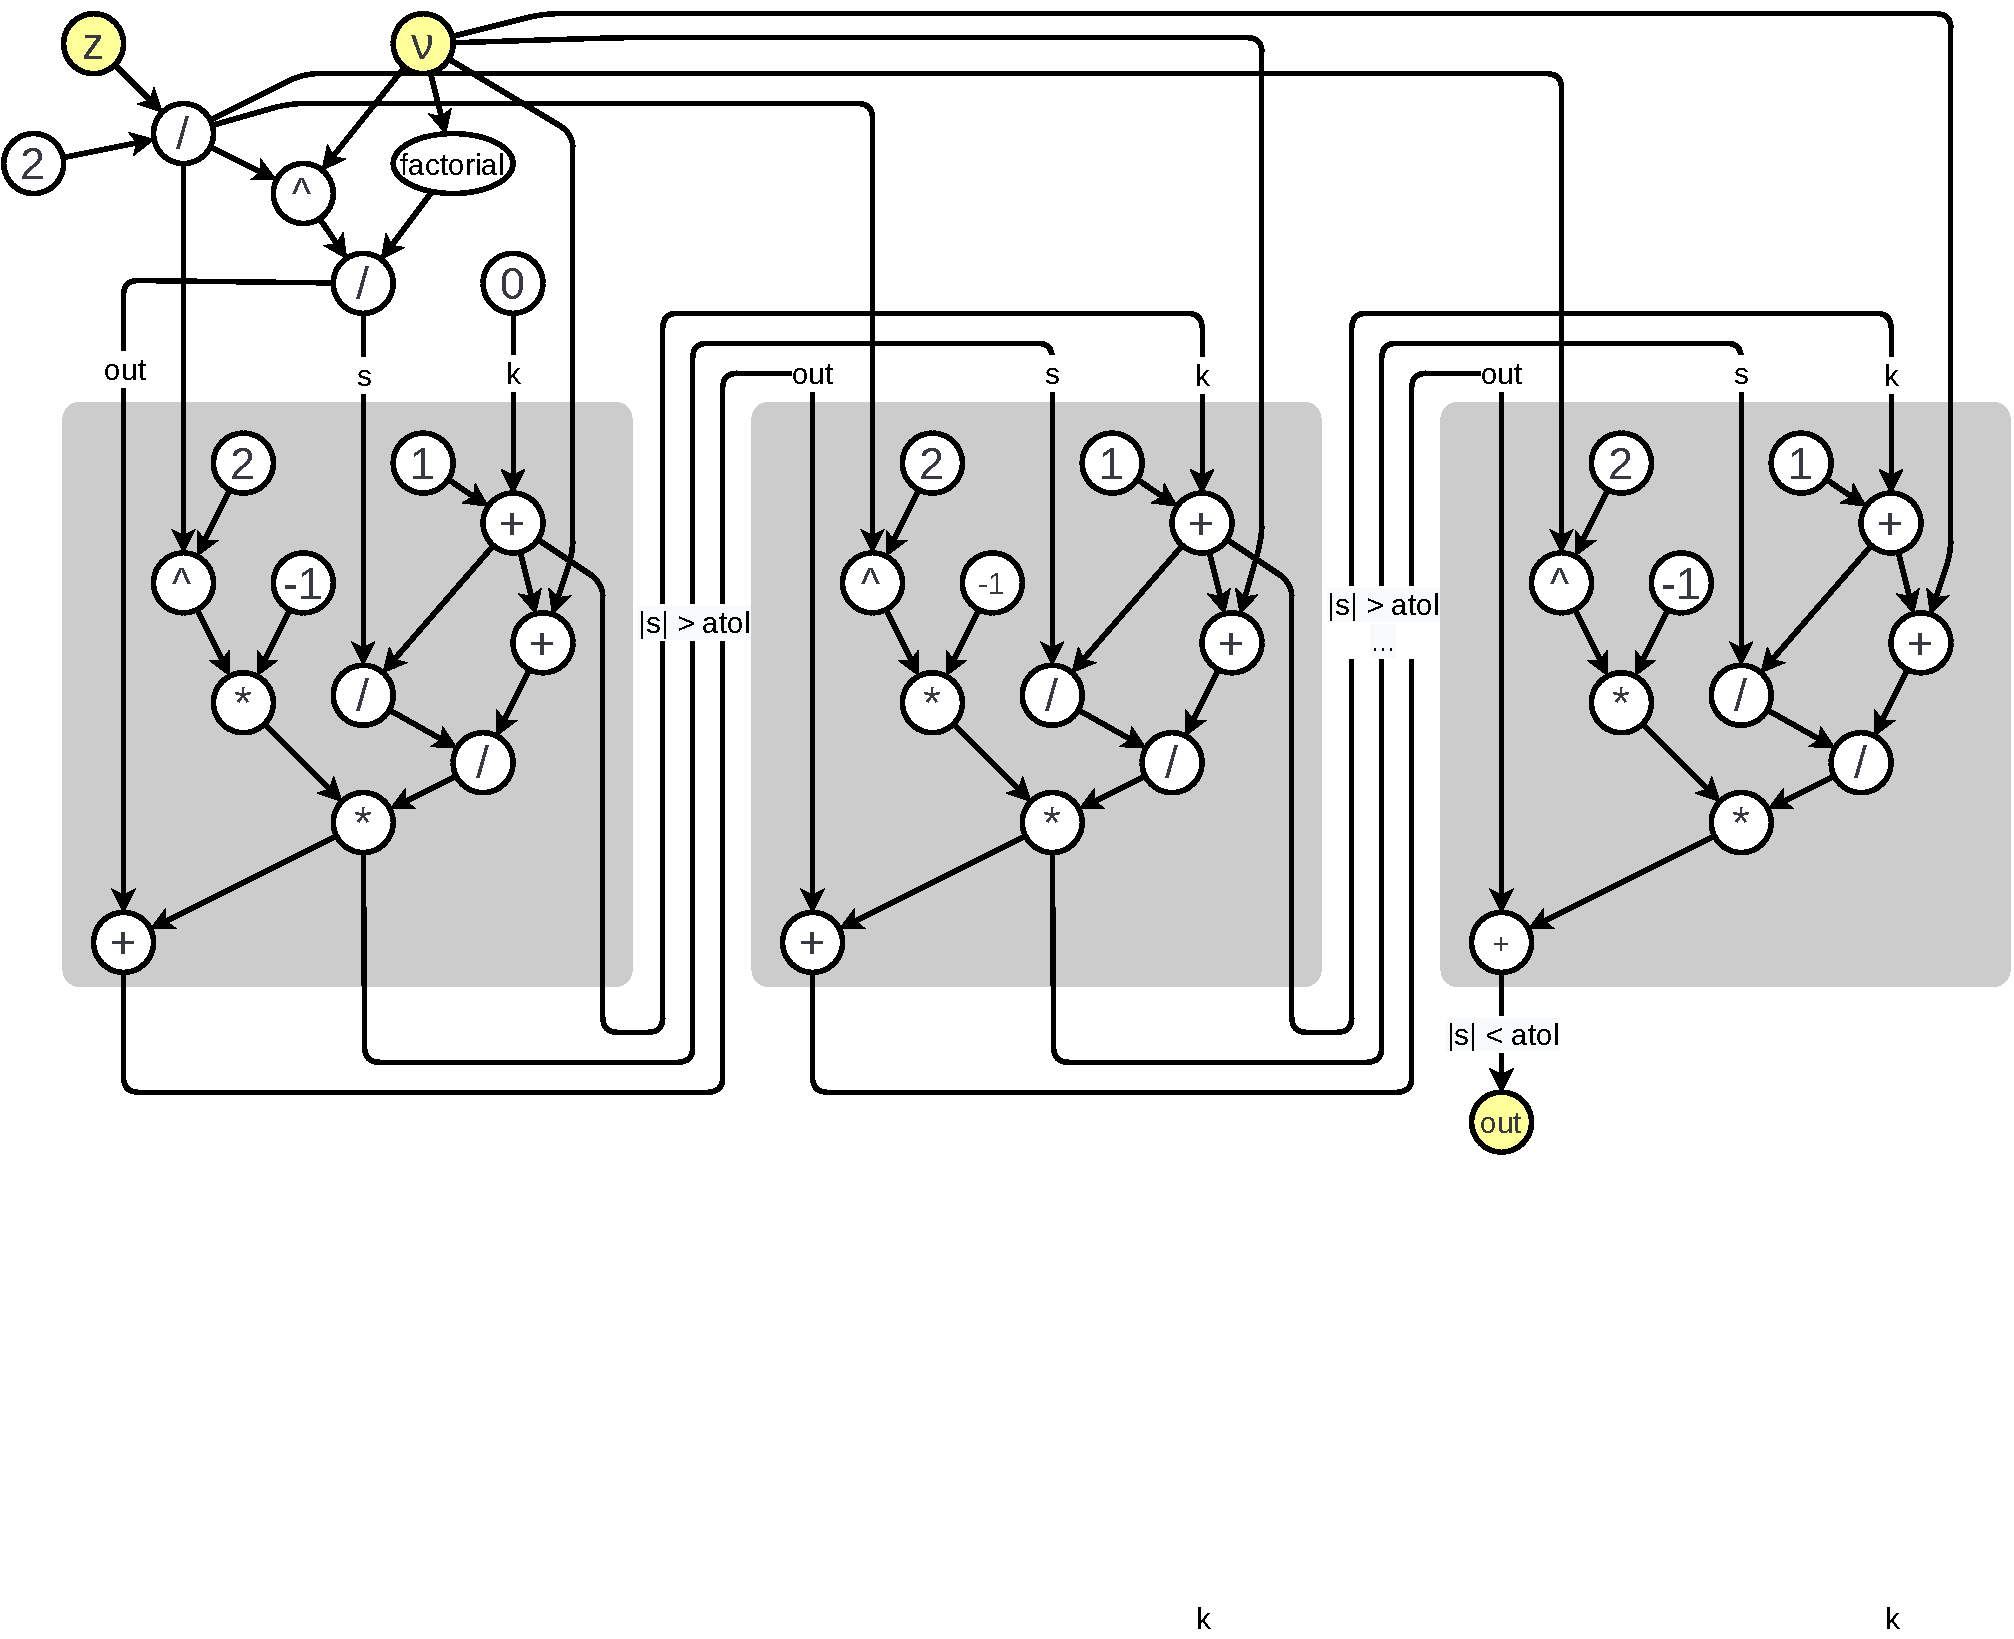
\includegraphics[width=\textwidth,trim={0 4cm 0 0cm},clip]{computational_graph.pdf}
        \caption{}
    \end{subfigure}%
    ~
    \begin{subfigure}[t]{0.47\textwidth}
        \centering
        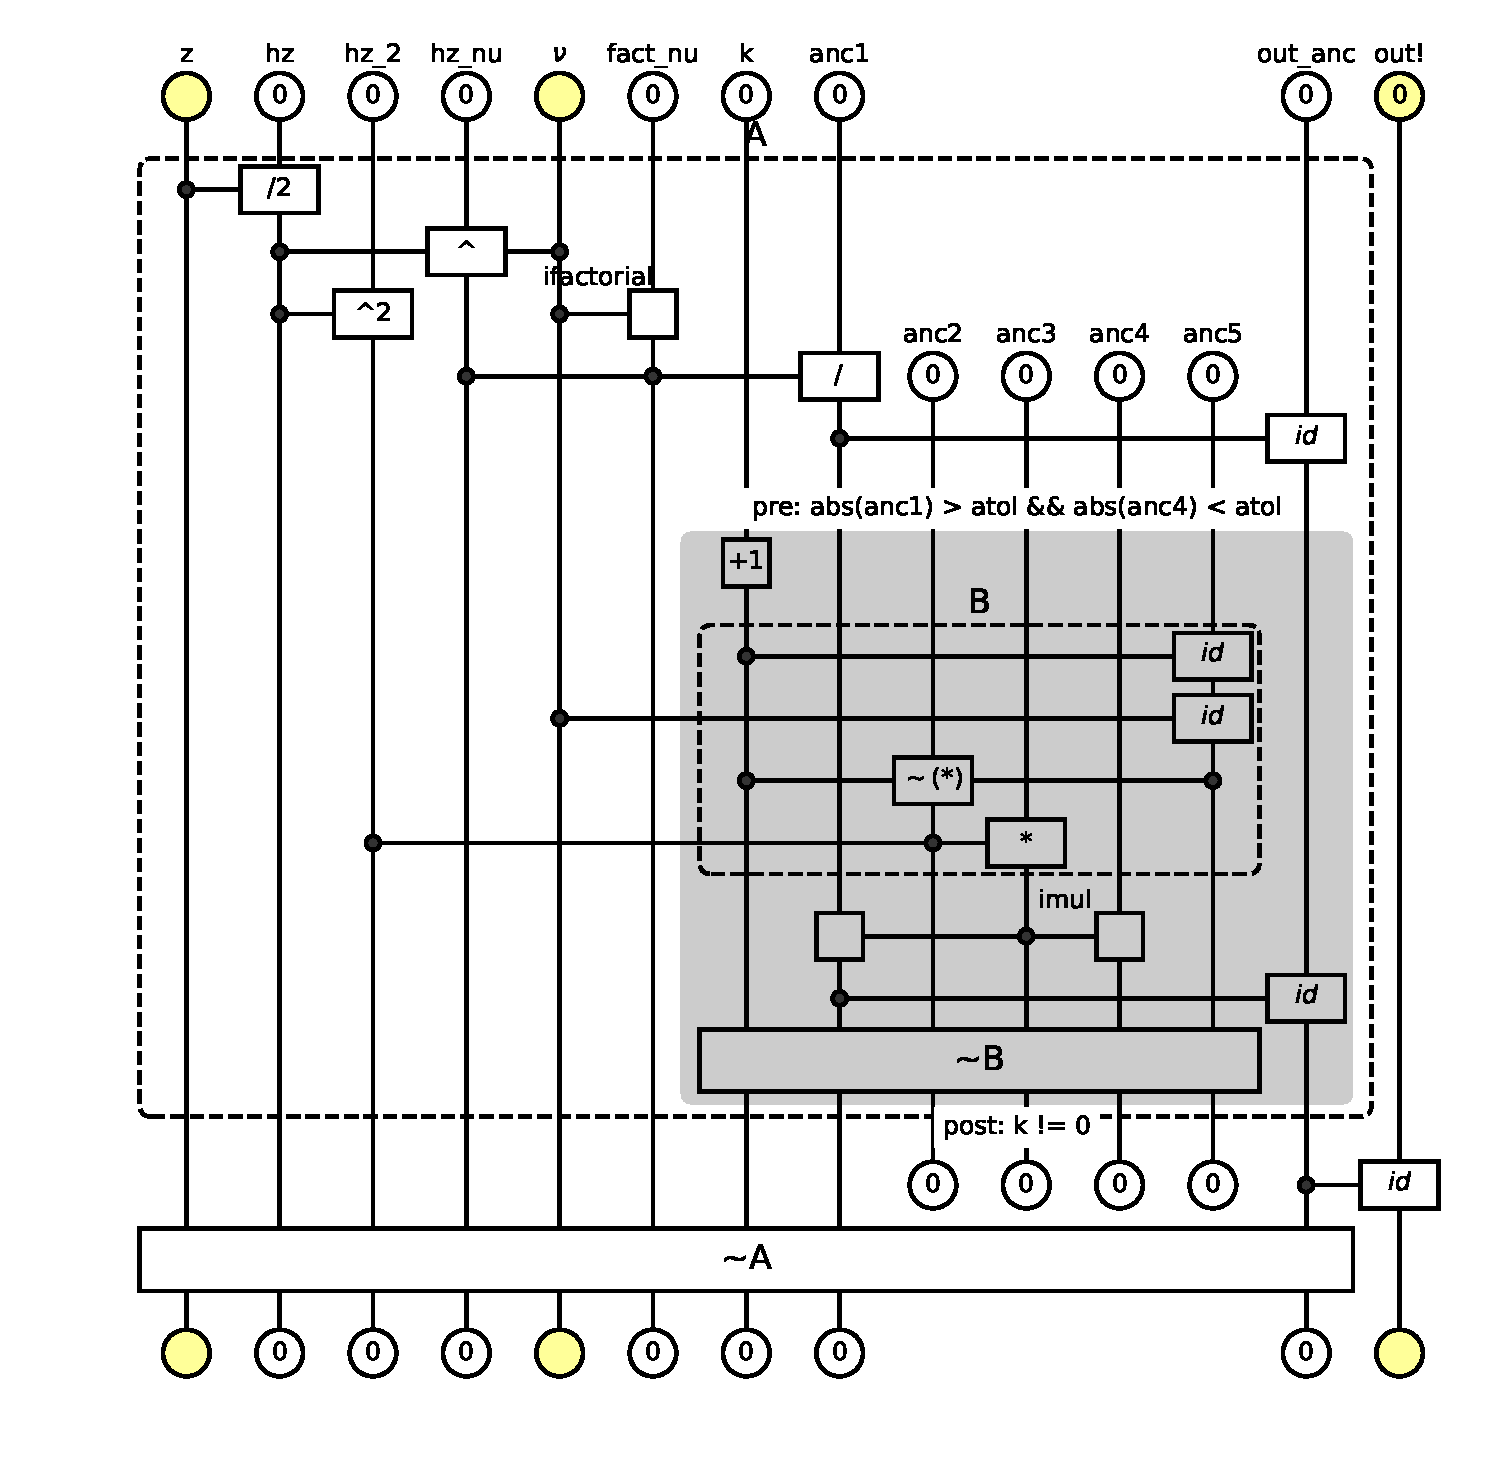
\includegraphics[width=\textwidth,trim={0 1cm 0 0cm},clip]{fig4.pdf}
        \caption{}
    \end{subfigure}
    \caption{(a) The traditional computational graph for the irreversible implementation of the first kind Bessel function. A vertex (circle) is an operation, and a directed edge is a variable. The gray regions are the body of the unrolled while loop.
        (b) The memory oriented computational graph for the reversible implementation of the first kind Bessel function. Notations are explained in \Fig{fig:ccu}.
    The gray region is the body of a while loop. Its precondition and postcondition are positioned on the top and bottom, respectively.
    }\label{fig:cgraphs}
\end{figure*}

Before showing the reversible implementation, we introduce how to obtain the product of a sequence of numbers reversibly.
Consecutive multiplication requires an increasing size of tape to cache an intermediate state $x_1 x_2 \ldots x_n$, since one can not deallocate the previous state $x_1 x_2 \ldots x_{n-1}$ directly since \texttt{*=} and \texttt{/=} are not considered as reversible here.
To mitigate the space overhead, the standard approach in reversible computing is the pebble game model~\cite{Perumalla2013} (or the checkpointing technique in machine learning),
where the cache size can be reduce in the cost of increasing the time complexity, however, constant cache size is not achievable in this scheme.
Hence, we introduce the following reversible approximate multiplier.

\begin{minipage}{.88\columnwidth}
    \begin{lstlisting}[numberstyle=\scriptsize\color{gray},numbers=left,numbersep=8pt]
@i @inline function imul(out!, x, anc!)
    anc! += out! * x
    out! -= anc! / x
    SWAP(out!, anc!)
end
\end{lstlisting}
\end{minipage}

Here, the third argument $\texttt{anc!}$ is a \textit{dirty ancilla}, which should be a value $\approx 0$.
Line 2 computes the result and accumulates it to the dirty ancilla, so that we have an approximate output in \texttt{anc!}.
Line 3 removes the content in \texttt{out!} approximately using the information stored in \texttt{anc!}.
Line 4 swaps the contents in \texttt{out!} and \texttt{anc!}.
Finally, we have an approximate output and a dirtier ancilla.
%The ``approximate uncomputing'' trick can be extensively used in practice. It mitigates the artificial irreversibility brought by the number system that we have adopted at the cost of output precision.
The reason why this trick works here lies in the fact that \texttt{*=} and \texttt{/=} are mathematically reversible (except the zero point) to each other.
One can approximately uncomputing the contents in the register at the cost of rounding errors.
This rounding error introduced in such a way only affects the function output, and does not sacrifice the reversibility.
With this approximate multiplier, we implement the reversible $J_\nu$ as follows.

\begin{minipage}{\columnwidth}
\begin{lstlisting}[multicols=2]
using NiLang, NiLang.AD

@i function ibesselj(out!, ν, z; atol=1e-8)
    k ← 0
    fact_nu ← zero(ν)
    halfz ← zero(z)
    halfz_power_nu ← zero(z)
    halfz_power_2 ← zero(z)
    out_anc ← zero(z)
    anc1 ← zero(z)
    anc2 ← zero(z)
    anc3 ← zero(z)
    anc4 ← zero(z)
    anc5 ← zero(z)

    @routine begin
        halfz += z / 2
        halfz_power_nu += halfz ^ ν
        halfz_power_2 += halfz ^ 2
        ifactorial(fact_nu, ν)

        anc1 += halfz_power_nu/fact_nu
        out_anc += identity(anc1)
        while (abs(unwrap(anc1))>atol && abs(unwrap(anc4)) < atol, k!=0)
            k += identity(1)
            @routine begin
                anc5 += identity(k)
                anc5 += identity(ν)
                anc2 -= k * anc5
                anc3 += halfz_power_2 / anc2
            end
            imul(anc1, anc3, anc4)
            out_anc += identity(anc1)
            ~@routine
        end
    end
    out! += identity(out_anc)
    ~@routine
end

@i function ifactorial(out!, n)
    anc ← zero(n)
    out! += identity(1)
    for i=1:n
        imul(out!, i, anc)
    end
end

@i @inline function imul(out!::T, x::T, anc!::T) where T<:Integer
    anc! += out! * x
    out! -= anc! ÷ x
    SWAP(out!, anc!)
end
\end{lstlisting}
\end{minipage}

The above algorithm uses a constant number of ancillas, while the time overhead is also a constant factor.
Ancilla \texttt{anc4} plays the role of \textit{dirty ancilla} in multiplication, and it is uncomputed rigorously in the uncomputing stage marked by \texttt{$\sim$@routine}.
This reversible program can be diagrammatically represented as a memory oriented computational graph as shown in \Fig{fig:cgraphs} (b).
This diagram can be used to analyze variables uncomputing. In this example, routine ``B'' uses \texttt{hz\_2}, \texttt{$\nu$} and \texttt{k} as control parameters, and changes the contents in \texttt{anc2}, \texttt{anc3} and \texttt{anc5}.
The following \texttt{imul} and \texttt{(:+=)(identity)} copies the result to output without changing these variables.
Hence we can apply the inverse routine \texttt{$\sim$B} to safely restore contents in \texttt{anc2}, \texttt{anc3} and \texttt{anc5}, and this examplifies the compute-copy-uncompute paradigm.

\begin{minipage}{.88\columnwidth}
\begin{lstlisting}
julia> out!, x = 0.0, 1.0
(0.0, 1.0)

julia> Grad(ibesselj)(Val(1), out!, 2, x)
(Val{1}(), GVar(0.0, 1.0), 2, GVar(1.0, 0.2102436))
\end{lstlisting}
\end{minipage}

One can obtain gradients of this function by calling \texttt{Grad(ibesselj)}.
Here, \texttt{Grad(ibesselj)} returns a callable instance of type \texttt{Grad\{typeof(ibesselj)\}}. The first parameters \texttt{Val(1)} specifies the position of loss in argument list. 
The Hessian can be obtained by feeding dual-numbers into this gradient function.

\begin{minipage}{.88\columnwidth}
\begin{lstlisting}
julia> out!, x = 0.0, 1.0
(0.0, 1.0)

julia> Grad(ibesselj)(Val(1), out!, 2, x)
(Val{1}(), GVar(0.0, 1.0), 2, GVar(1.0, 0.2102436))

julia> using ForwardDiff: Dual

julia> _, hxout!, _, hxx = Grad(ibesselj)(Val(1), 
        Dual(out!, zero(out!)), 2, Dual(x, one(x)));

julia> grad(hxx).partials[1]
0.13446683844358093
\end{lstlisting}
\end{minipage}

Here, the gradient field of \texttt{hxx} is defined as $\frac{\partial {\rm out!}}{\partial x}$, which is a Dual number.
It has a field \texttt{partials} that store the Hessian $\frac{\partial{\rm out!}^2}{\partial x^2}$.

\subsection{Solving a graph embedding problem}\label{sec:graph}
Graph embedding can be used to find a proper representation for an order parameter~\cite{Takahashi2020} in condensed matter physics.
\Ref{Takahashi2020} considers a problem of finding the minimum Euclidean space dimension $k$ that a Petersen graph can embed into, that the distances between pairs of connected vertices are $l_1$, and the distance between pairs of disconnected vertices are $l_2$, where $l_2 > l_1$.
The Petersen graph is shown in \Fig{fig:petersen}.
Let us denote the set of connected and disconnected vertex pairs as $L_1$ and $L_2$, respectively. This problem can be variationally solved with the following loss.
\begin{align}
    \begin{split}
        \mathcal{L} &= \Var({\rm dist}(L_1)) + \Var({\rm dist}(L_2)) \\
        &+\exp({\rm relu}(\overline{{\rm dist}(L_1)} - \overline{{\rm dist}(L_2)} + 0.1))) - 1
    \end{split}
\end{align}
The first line is a summation of distance variances in two sets of vertex pairs, where $\Var(X)$ is the variance of samples in $X$.
The second line is used to guarantee $l_2 > l_1$, where $\overline{X}$ means taking the average of samples in $X$.
Its reversible implementation could be found in our benchmark repository.

We repeat the training for dimension $k$ from $1$ to $10$.
In each training, we fix two of the vertices and optimize the positions of the rest. Otherwise, the program will find the trivial solution with overlapped vertices. 
For $k < 5$, the loss is always much higher than $0$,
while for $k\geq5$, we can get a loss close to machine precision with high probability.
From the $k=5$ solution, it is easy to see $l_2/l_1 = \sqrt{2}$.
An Adam optimizer with a learning rate $0.01$~\cite{Kingma2014} requires $\sim2000$ steps training.
The trust region Newton's method converges much faster, which requires $\sim 20$ computations of Hessians to reach convergence.
Although training time is comparable, the converged precision of the later is much better.
\begin{figure}
    \centerline{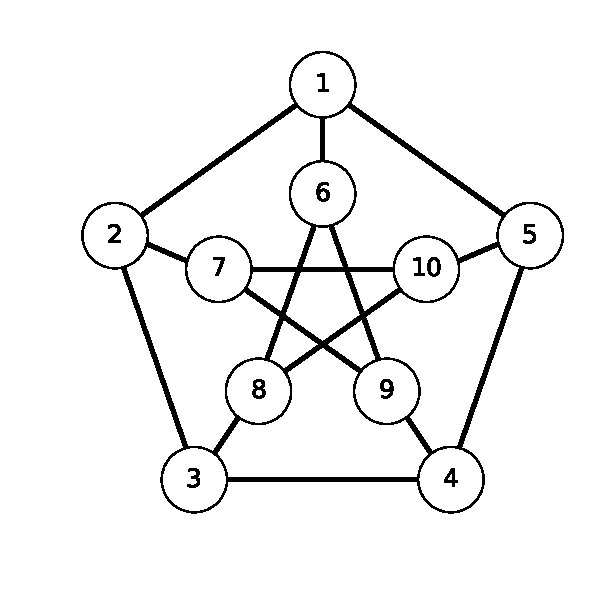
\includegraphics[width=0.4\columnwidth,trim={0 1cm 0 0},clip]{petersen.pdf}}
    \caption{The Petersen graph has 10 vertices and 15 edges. We want to find a minimum embedding dimension for it.}\label{fig:petersen}
\end{figure}


\section{Benchmarks}\label{sec:benchmark}

In the following benchmarks the CPU device is Intel(R) Xeon(R) Gold 6230 CPU @ 2.10GHz, and the GPU device is Nvidia Titan V.
% the GPU time is estimated by broadcasting the gradient function on CUDA array of size $2^{17}$ and taking the average.
For NiLang benchmarks, we have turned off the reversibility check off to achieve a better performance.

\subsection{Sparse matrices}\label{sec:benchsparse}
We benchmarked the call, uncall and backward propagation time used for sparse matrix dot product and matrix multiplication.
Here, we estimate the time for back propagating gradients rather than including both forward and backward, since \texttt{mul!} does not output a scalar as loss.

\begin{table}[h!]\centering
\begin{minipage}{0.8\columnwidth}
\ra{1.3}
    \scalebox{1.0}{
        \begin{tabularx}{\textwidth}{bsb}\toprule
            \textbf{}     & \texttt{dot}         & \texttt{mul!} (complex valued) \\
            \hline
            Julia-O       & 3.493e-04   & 8.005e-05\\
            NiLang-O      & 4.675e-04   & 9.332e-05\\
            \hline
            NiLang-B      & 5.821e-04   & 2.214e-04\\
            \bottomrule
        \end{tabularx}
    }
    \caption{Absolute runtimes in seconds for computing the objectives (O) and the backward pass (B) of sparse matrix operations. The matrix size is $1000 \times 1000$, and the element density is $0.05$. The total time used in computing gradient can be estimated as a sum of ``O'' and ``B''.
    }\label{tbl:sparse}
\end{minipage}
\end{table}

The time used for computing backward pass is approximately 1.5-3 times the Julia's native forward pass.
This is because the instruction length of differentiating basic arithmetic instructions is longer than pure computing by a factor of 2 or more.


\subsection{Bessel Function}\label{sec:besselbench}
We differentiate the first type Bessel function in \Sec{sec:bessel} and show the benchmarks in \Tbl{tbl:besselj}.
In the table, Julia is the CPU time used for running the irreversible forward program. It is the baseline for benchmarking.
NiLang (call/uncall) is the time of reversible call or uncall. Both of them are $\sim2$ times slower than its irreversible counterpart. Since Bessel function has only one input argument, forward mode AD tools are faster than reverse mode AD, both source-to-source framework ForwardDiff and operator overloading framework Tapenade have the a comparable computing time with the pure function call.
\begin{table}[h!]\centering
\begin{minipage}{0.8\columnwidth}
\ra{1.3}
    \scalebox{1.0}{
        \begin{tabularx}{\textwidth}{X X c}\toprule
            & $T_{\rm min}$/ns & Space/KB\\
            \hline
            Julia-O & 18 & 0\\
            NiLang-O & 32 & 0\\
            Tapenade-O & 32 & 0\\
            \hline
            ForwardDiff-G & 38 & 0\\
            %Manual & Backward & 83 & 0\\
            NiLang-G & 201 & 0\\
            NiLang-G (CUDA) & 1.4 & 0\\
            ReverseDiff-G & 1406 & 1.2\\
            Zygote-G & 22596 & 13.47\\
            Tapenade-G (Forward) & 30 & 0\\
            Tapenade-G (Backward) & 111 & > 0\\
            \bottomrule
        \end{tabularx}
    }
    \caption{Time and space used for computing objective (O) and gradient (G) of the first kind Bessel function $J_2(1.0)$.
    The CUDA benchmark time is averaged over a batch size of 4000, which is not a fair comparison but shows how much performance can we get from GPU in the parallel computing context.
}\label{tbl:besselj}
\end{minipage}
\end{table}

NiLang.AD is the reverse mode AD submodule in NiLang, and it takes ~11 times the native Julia program, and is also 2 times slower than Tapenade. However, the key point is, there is no extra memory allocation like stack operations in the whole computation. The controllable memory allocation of NiLang makes it compatible with CUDA program.
%For people who are interested in CUDA programming, we prepared another example in \App{app:cuda}, which implements a differentiable quantum simulation kernel on GPU.
%So far, the generated backward rule faces the shared write problem, which requires further investigation.
%, and 
In other backward mode AD like Zygote, ReverseDiff and Tapenade, the memory allocation in heap is nonzero due to the checkpointing.

\subsection{Graph embedding problem}\label{sec:graphbench}
Since one can combine ForwardDiff and NiLang to obtain Hessians,
it is interesting to see how much performance we can get in differentiating the graph embedding program in \Sec{sec:graph}.

\begin{table}[h!]\centering
    \small
\begin{minipage}{\columnwidth}
\ra{1.3}
    \scalebox{1.0}{
        \begin{tabularx}{\textwidth}{bssssssssss}\toprule
            $k$                      & 2          & 4          & 6          & 8          & 10         \\
            \hline
            Julia-O                  & 4.477e-06  & 4.729e-06  & 4.959e-06  & 5.196e-06  & 5.567e-06  \\
            NiLang-O                 & 7.173e-06  & 7.783e-06  & 8.558e-06  & 9.212e-06  & 1.002e-05  \\
            NiLang-U                 & 7.453e-06  & 7.839e-06  & 8.464e-06  & 9.298e-06  & 1.054e-05  \\
            \hline
            NiLang-G                 & 1.509e-05  & 1.690e-05  & 1.872e-05  & 2.076e-05  & 2.266e-05  \\
            ReverseDiff-G            & 2.823e-05  & 4.582e-05  & 6.045e-05  & 7.651e-05  & 9.666e-05  \\
            ForwardDiff-G            & 1.518e-05  & 4.053e-05  & 6.732e-05  & 1.184e-04  & 1.701e-04  \\
            Zygote-G                 & 5.315e-04  & 5.570e-04  & 5.811e-04  & 6.096e-04  & 6.396e-04  \\
            \hline
            (NiLang+F)-H             & 4.528e-04  & 1.025e-03  & 1.740e-03  & 2.577e-03  & 3.558e-03  \\
            ForwardDiff-H            & 2.378e-04  & 2.380e-03  & 6.903e-03  & 1.967e-02  & 3.978e-02  \\
            (ReverseDiff+F)-H        & 1.966e-03  & 6.058e-03  & 1.225e-02  & 2.035e-02  & 3.140e-02  \\
            \bottomrule
        \end{tabularx}
    }
    \caption{Absolute times in seconds for computing the objectives (O), uncall objective (U), gradients (G) and Hessians (H) of the graph embedding program.
    $k$ is the embedding dimension, the number of parameters is $10k$.
    }\label{tbl:graphembedding}
\end{minipage}
\end{table}

In \Tbl{tbl:graphembedding}, we show the the performance of different implementations by varying the dimension $k$. The number of parameters is $10k$.
As the baseline, (a) shows the time for computing the function call. We have reversible and irreversible implementations, where the reversible program is slower than the irreversible native Julia program by a factor of $\sim2$ due to the uncomputing overhead.
The reversible program shows the advantage of obtaining gradients when the dimension $k \geq 3$. The larger the number of inputs, the more advantage it shows due to the overhead proportional to input size in forward mode AD.
The same reason applies to computing Hessians, where the combo of NiLang and ForwardDiff gives the best performance for $k \geq 3$.

\subsection{Gaussian mixture model and bundle adjustment}\label{sec:ba}

We reproduced the benchmarks for Gaussian mixture model (GMM) and bundle adjustment (BA) in ~\Ref{Srajer2018} by re-writing the programs in a reversible style. We show the results in \Tbl{tbl:gmm} and \Tbl{tbl:ba}. In our new benchmarks, we also rewrite the ForwardDiff program for a fair benchmark, this explains the difference between our results and the original benchmark. The Tapenade data is obtained by executing the docker file provided by the original benchmark, which provides a baseline for comparison.

\begin{table}[h!]\centering
    \scriptsize
\begin{minipage}{\columnwidth}
\ra{1.3}
    \scalebox{1.0}{
        \begin{tabularx}{\textwidth}{bssssssss}\toprule
            \textbf{\# parameters} & 3.00e+1 & 3.30e+2 & 1.20e+3 & 3.30e+3 & 1.07e+4 & 2.15e+4 & 5.36e+4 & 4.29e+5\\
            \hline
            Julia-O       & 9.844e-03 & 1.166e-02 & 2.797e-01 & 9.745e-02 & 3.903e-02 & 7.476e-02 & 2.284e-01 & 3.593e+00  \\
            NiLang-O      & 3.655e-03 & 1.425e-02 & 1.040e-01 & 1.389e-01 & 7.388e-02 & 1.491e-01 & 4.176e-01 & 5.462e+00  \\
            Tapende-O     & 1.484e-03 & 3.747e-03 & 4.836e-02 & 3.578e-02 & 5.314e-02 & 1.069e-01 & 2.583e-01 & 2.200e+00\\
            \hline
            ForwardDiff-G & 3.551e-02 & 1.673e+00 & 4.811e+01 & 1.599e+02 & -         & -         & -         & -  \\
            NiLang-G      & 9.102e-03 & 3.709e-02 & 2.830e-01 & 3.556e-01 & 6.652e-01 & 1.449e+00 & 3.590e+00 & 3.342e+01  \\
            Tapenade-G    & 5.484e-03 & 1.434e-02 & 2.205e-01 & 1.497e-01 & 4.396e-01 & 9.588e-01 & 2.586e+00 & 2.442e+01\\
            \bottomrule
        \end{tabularx}
    }
    \caption{Absolute runtimes in seconds for computing the objective (O) and gradients (G) of GMM with 10k data points. ``-'' represents missing data due to not finishing the computing in limited time.}\label{tbl:gmm}
\end{minipage}
\end{table}

In the GMM benchmark, NiLang's objective function has overhead comparing with irreversible programs in most cases.
Except the uncomputing overhead, it is also because our naive reversible matrix-vector multiplication is much slower than the highly optimized BLAS function, where the matrix-vector multiplication is the bottleneck of the computation.
The forward mode AD suffers from too large input dimension in the large number of parameters regime.
Although ForwardDiff batches the gradient fields, the overhead proportional to input size still dominates.
The source to source AD framework Tapenade is faster than NiLang in all scales of input parameters,
but the ratio between computing the gradients and the objective function are close.
%The memory consumption of our reversible implementation is quite low.
%The peak memory is only slightly more than twice of the original program,
%where the factor 2 comes from wrapping each variable with an extra gradient field.

\begin{table}[h!]\centering
    \scriptsize
\begin{minipage}{\columnwidth}
\ra{1.3}
    \scalebox{1.0}{
        \begin{tabularx}{\textwidth}{bsssssss}\toprule
            \textbf{\# measurements} & 3.18e+4 & 2.04e+5 & 2.87e+5 & 5.64e+5 & 1.09e+6 & 4.75e+6 & 9.13e+6\\
            \hline
            Julia-O        & 2.020e-03 & 1.292e-02 & 1.812e-02 & 3.563e-02 & 6.904e-02 & 3.447e-01 & 6.671e-01\\
            NiLang-O       & 2.708e-03 & 1.757e-02 & 2.438e-02 & 4.877e-02 & 9.536e-02 & 4.170e-01 & 8.020e-01\\
            Tapenade-O     & 1.632e-03 & 1.056e-02 & 1.540e-02 & 2.927e-02 & 5.687e-02 & 2.481e-01 & 4.780e-01\\
            \hline
            ForwardDiff-J  & 6.579e-02 & 5.342e-01 & 7.369e-01 & 1.469e+00 & 2.878e+00 & 1.294e+01 & 2.648e+01\\
            NiLang-J       & 1.651e-02 & 1.182e-01 & 1.668e-01 & 3.273e-01 & 6.375e-01 & 2.785e+00 & 5.535e+00\\
            NiLang-J (GPU) & 1.354e-04 & 4.329e-04 & 5.997e-04 & 1.735e-03 & 2.861e-03 & 1.021e-02 & 2.179e-02\\
            Tapenade-J     & 1.940e-02 & 1.255e-01 & 1.769e-01 & 3.489e-01 & 6.720e-01 & 2.935e+00 & 6.027e+00\\
            \bottomrule
        \end{tabularx}
    }
    \caption{Absolute runtimes in seconds for computing the objective (O) and Jacobians (J) in bundle adjustment.}\label{tbl:ba}
\end{minipage}
\end{table}

In the BA benchmark, reverse mode AD shows slight advantage over ForwardDiff.
The bottleneck of computing this large sparse Jacobian is computing the Jacobian of a elementary function with 15 input arguments and 2 output arguments, where input space is larger than the output space.
In this instance, our reversible implementation is even faster than the source code transformation based AD framework Tapenade.
With KernelAbstractions, we run our zero allocation reversible program on GPU, which provides a >200x speed up.
%Running codes on GPU (in Julia) requires not introducing any memory allocation at the kernel level.
%NiLang provides user the flexibility to manage the memory allocation instead of using a global stack.

\section{Discussion and outlooks}\label{sec:discussion}
In this paper, we show how to realize a reversible programming eDSL and implement an instruction level backward mode AD on top of it.
It gives the user more flexibility to tradeoff memory and computing time comparing with traditional checkpointing.
The Julia implementation NiLang gives the state-of-the-art performance and memory efficiency in obtaining first and second-order gradients in applications, including first type Bessel function, sparse matrix manipulations, solving graph embedding problem, Gaussian mixture model and bundle adjustment.
%In a reversible programming language, we proposed to use ``approximate uncomputing'' trick to avoid the overhead of a reversible program in many practical cases.

In the following, we discuss some practical issues about reversible programming, and several future directions to go.
%Notablely, we introduce the concept of ``arithematic uncomputing'' to reduce the overhead of recursive reversible algorithms.

\subsection{Time Space Tradeoff}\label{sec:timespace}
In history, there have been many discussions about time-space tradeoff on a reversible Turing machine (RTM).
In the most straightforward g-segment tradeoff scheme~\cite{Bennett1989,Levine1990}, an RTM model has either a space overhead that is proportional to computing time $T$ or a computational overhead that sometimes can be exponential to the program size comparing with an irreversible counterpart.
This result stops many people from taking reversible computing seriously as a high-performance computing scheme.
In the following, we try to explain why the overhead of reversible computing is not as terrible as people thought.

First of all, the overhead of reversing a program is upper bounded by the checkpointing~\cite{Chen2016} strategy used in many traditional machine learning package that memorizes inputs of primitives because checkpointing can be trivially implemented in reversible programming.~\cite{Perumalla2013} 
Reversible programming provides some alternatives to reduce the overhead.
For example, accumulation is reversible, so that many BLAS functions can be implemented reversiblly without extra memory.
Meanwhile, the memory allocation in some iterative algorithms can often be reduced with the ``arithmetic uncomputing'' trick without sacrificing reversibility, as shown in the \texttt{ibesselj} example in \Sec{sec:bessel}.
Clever compiling based on memory oriented computational graphs (\Fig{fig:ccu} and \Fig{fig:cgraphs} (b)) can also be used to help user tradeoff between time and space.
The overhead of a reversible program mainly comes from the uncomputing of ancillas.
It is possible to automatically uncompute ancillas by analyzing variable dependency instead of asking users to write \texttt{@routine} and \texttt{$\sim$@routine} pairs.
In a hierarchical design, uncomputing can appear in every memory deallocation (or symbol table reduction). To quantify the overhead of uncomputing, we introduce the term uncomputing level as bellow.
\begin{definition}[uncomputing level]
    The log-ratio between the number of instructions of a reversible program and its irreversible counterpart.
\end{definition}
From the lowest instruction level, whenever we reduce the symbol table (or space), the computational cost doubles.
The computational overhead grows exponentially as the uncomputating level increases, which can be seen from some of the benchmarks in the main text.
In sparse matrix multiplication and dot product, we don't introduce uncomputing in the most time consuming part, so it is $\sim0$. The space overhead is \texttt{2*m} to keep the branch decisions, which is even much smaller than the memory used to store row indices.
in Gaussian mixture model, the most time consuming matrix-vector multiplication is doubled, so it is $\sim 1$. The extra memory usage is approximately 0.5\% of the original program.
In the first kind Bessel function and bundle adjustment program, the most time consuming parts are (nestedly) uncomputed twice, hence their uncomputing level is $\sim2$.
Such aggressive uncomputing makes zero memory allocation possible.
%At last, making reversible programming an eDSL rather than an independent language allows flexible choices between reversibility and computational overhead. For example, to deallocate the memory that stores gradients in a reversible language, one has to uncompute the whole process of obtaining them.
%As an eDSL, one has an alternative to deallocate the memory irreversibly outside the scope of a reversible program, i.e., trade energy with time.

\subsection{Differentiability as a Hardware Feature}\label{sec:hardware}

\begin{figure}
    \centerline{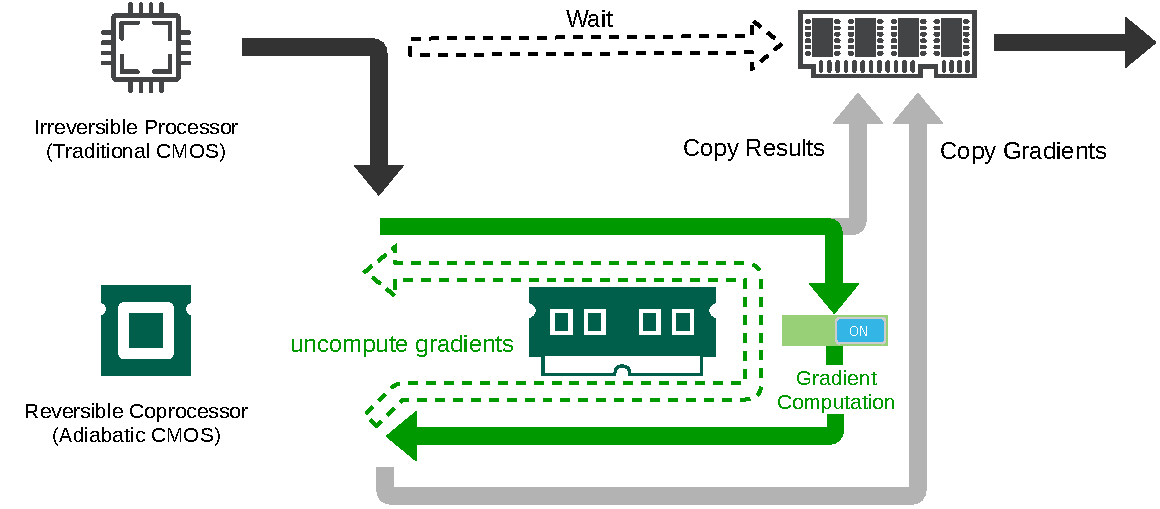
\includegraphics[width=0.8\columnwidth,trim={0 0cm 0 0cm},clip]{hardware.pdf}}
    \caption{Energy efficient AI co-processor. Green arrows represents energy efficient operations on reversible devices.}\label{fig:hardware}
\end{figure}
So far, our eDSL is compiled to Julia language. It relies on Julia's multiple dispatch to differentiate a program, which requires users to write generic programs.
A more liable AD should be a hardware or micro instruction level feature.
In the future, we can expect NiLang being compiled to reversible instructions~\cite{Vieri1999} and executed on a reversible device.
A reversible devices can play a role of differentiation engine as shown in the hetero-structural design in \Fig{fig:hardware}.
It defines a reversible instruction set and has a switch that controls whether the instruction calls a normal instruction or an instruction that also updates gradients.
When a program calls a reversible differentiable subroutine, the reversible co-processor first marches forward, compute the loss and copy the result to the main memory.
Then the co-processor execute the program backward and uncall instructions, initialize and updating gradient fields at the same time.
After reaching the starting point of the program, the gradients are transferred to the global memory.
Running AD program on a reversible device can save energy. Theoretically, the reversible routines do not necessarily cost energy, the only energy bottleneck is copying gradient and outputs to the main memory.

\subsection{The connection to Quantum programming}
A Quantum device~\cite{Nielsen2002} is a special reversible hardware that features quantum entanglement.
The instruction set of classical reversible programming is a subset of quantum instruction set.
However, building a universal quantum computer is difficult. 
Unlike a classical state, a quantum state can not be cloned. Meanwhile, it loses information by interacting with the environment.
Classical reversible computing does not enjoy the quantum advantage, nor the quantum disadvantages of non-cloning and decoherence,
but it is a model that we can try directly with our classical computer.
It is technically smooth to have a reversible computing device to bridge the gap between classical devices and universal quantum computing devices.
By introducing entanglement little by little, we can accelerate some elementary components in reversible computing. For example, quantum Fourier transformation provides an alternative to the reversible adders and multipliers by introducing the Hadamard and CPHASE quantum gates~\cite{RuizPerez2017}.
From the programming languages's perspective, most quantum programming language preassumes the existence of a classical coprocessor to control quantum devices~\cite{Svore2018}.
It is also interesting to know what is a native quantum control flow like, and does quantum entanglement provide speed up to automatic differentiation?
We believe the reversible compiling technologies will open a door to study quantum compiling.

\subsection{Gradient on ancilla problem}
In this subsection, we introduce an easily overlooked problem in our reversible AD framework.
An ancilla can sometimes carry a nonzero gradient when it is deallocated. As a result, the gradient program can be irreversible in the local scope.
In NiLang, we drop the gradient field of ancillas instead of raising an error.
In the following, we justify our decision by proving the following theorem.
\begin{theorem}
    Deallocating an ancilla with constant value field and nonzero gradient field does not introduce incorrect gradients.
\end{theorem}
\begin{proof}
    Consider a reversible function $\vx^i, b = f_i(\vx^{i-1}, a)$, where $a$ and $b$ are the input and output values of an ancilla.
    Since both $a$, $b$ are constants that are independent of input $\vx^{i-1}$, we have
\begin{align}
    \frac{\partial b}{\partial \vx^{i-1}} = \mathbf{0}.
\end{align}
Discarding gradients should not have any effect on the \texttt{value} fields of outputs.
    The key is to show $\texttt{grad(b)} \equiv \frac{\partial \vx^L}{\partial{b}}$ does appear in the \texttt{grad} fields of the output. It can be seen from the back-propagation rule 
\begin{equation}
    \frac{\partial \vx^L}{\partial \vx^{i-1}} = \frac{\partial \vx^L}{\partial \vx^i}\frac{\partial \vx^i}{\partial \vx^{i-1}} + \frac{\partial \vx^L}{\partial b}\frac{\partial b}{\partial \vx^{i-1}},
\end{equation}
where the second term with $\frac{\partial \vx^L}{\partial{b}}$ vanishes naturally. We emphasis here, the value part of discarded ancilla must be a constant.
\end{proof}

\subsection{Shared read and write problem}\label{sec:sharedrw}
One should be careful about shared read in reversible programming AD, because the shared read can introduce shared write in the adjoint program.
Let's begin with the following expression.

\begin{minipage}{.88\columnwidth}
\begin{lstlisting}
y += x * y
\end{lstlisting}
\end{minipage}

Most people will agree that this statement is not reversible and should not be allowed because it changes input variables.
We call it the \textit{simultaneous read-and-write} issue.
However, the following expression with two same inputs is a bit subtle.

\begin{minipage}{.88\columnwidth}
\begin{lstlisting}
y += x * x
\end{lstlisting}
\end{minipage}

It is reversible, but should not be allowed in an AD program because of the \textit{shared write} issue.
It can be seen directly from the expanded expression.

\begin{minipage}{.88\columnwidth}
\begin{lstlisting}
julia> macroexpand(Main, :(@instr y += x * x))
quote
    var"##253" = ((PlusEq)(*))(y, x, x)
    begin
        y = ((NiLangCore.wrap_tuple)(var"##253"))[1]
        x = ((NiLangCore.wrap_tuple)(var"##253"))[2]
        x = ((NiLangCore.wrap_tuple)(var"##253"))[3]
    end
end
\end{lstlisting}
\end{minipage}

In an AD program, the gradient field of \texttt{x} will be updated.
The later assignment to $x$ will overwrite the former one and introduce an incorrect gradient.
One can get free of this issue by avoiding using same variable in a single instruction

\begin{minipage}{.88\columnwidth}
\begin{lstlisting}
anc ← zero(x)
anc += identity(x)
y += x * anc
anc -= identity(x)
\end{lstlisting}
\end{minipage}

or equivalently,

\begin{minipage}{.88\columnwidth}
\begin{lstlisting}
y += x ^ 2
\end{lstlisting}
\end{minipage}

Share variables in an instruction can be easily identified and avoided.
However, it becomes tricky when one runs the program in a parallel way.
For example, in CUDA programming, every thread may write to the same gradient field of a shared scalar.
How to solve the shared write in CUDA programming is still an open problem, which limits the power of reversible programming AD on GPU.

\subsection{Outlook}\label{sec:outlook}

We can use NiLang to solve some existing issues related to AD.
Reversible programming can make use of reversibility to save memory.
Reversibility has been used in reducing the memory allocations in machine learning models such as recurrent neural networks~\cite{MacKay2018}, Hyperparameter learning~\cite{Maclaurin2015} and residual neural networks~\cite{Behrmann2018}.
We can use it to generate AD rules for existing machine learning packages like \href{https://github.com/JuliaDiff/ReverseDiff.jl}{ReverseDiff}, Zygote~\cite{Innes2019}, Knet~\cite{Yuret2016}, and Flux~\cite{Innes2018a}.
Many backward rules for sparse arrays and linear algebra operations have not been defined yet in these packages.
We can also use the flexible time-space tradeoff in reversible programming to overcome the memory wall problem in some applications.
A successful, related example is the memory-efficient domain-specific AD engine in quantum simulator Yao~\cite{Luo2019}.
This domain-specific AD engine is written in a reversible style and solved the memory bottleneck in variational quantum simulations. It also gives so far the best performance in differentiating quantum circuit parameters.
Similarly, we can write memory-efficient normalizing flow~\cite{Kobyzev2019} in a reversible style. Normalizing flow is a successful class of generative models in both computer vision~\cite{Kingma2018} and quantum physics~\cite{Dinh2016,Li2018}, where its building block bijector is reversible.
We can use a similar idea to differentiate reversible integrators~\cite{Hut1995, Laikov2018}.
With reversible integrators, it should be possible to rewrite the control system in robotics~\cite{Giftthaler2017} in a reversible style, where scalar is a first-class citizen rather than tensor.
Writing a reversible control program should boost training performance.
Reversibility is also a valuable resource for training.

To solve the above problems better, reversible programming should be improved from multiple perspectives.
First, we need a better compiler for compiling reversible programs.
To be specific, a compiler that admits mutability of data, and handle shared read and write better.
Then, we need a reversible number system and instruction set to avoid rounding errors and support reversible control flows better.
There are proposals of reversible floating point adders and multipliers, however these designs require allocating garbage bits in each operation~\cite{Nachtigal2010,Nachtigal2011,Nguyen2013,Hner2018}.
In NiLang, one can simulate rigorous reversible arithmetic with the fixed-point number package \href{https://github.com/JuliaMath/FixedPointNumbers.jl}{FixedPointNumbers}.
However, a more efficient reversible design requires instruction-level support.
Some other numbers systems are reversible under \texttt{*=} and \texttt{/=} rather than \texttt{+=} and \texttt{-=}, including \href{https://github.com/cjdoris/LogarithmicNumbers.jl}{LogarithmicNumbers}~\cite{Taylor1988} and \href{https://github.com/GiggleLiu/TropicalNumbers.jl}{TropicalNumbers}.
They are powerful tools to solve domain specific problems, for example, we have an upcoming work about differentiating over tropical numbers to solve the ground state configurations of a spinglass system efficiently.
We also need \texttt{comefrom} like instruction as a partner of \texttt{goto} to specify the postconditions in our instruction set.
Finally, although we introduced that the adiabatic CMOS as a better choice as the computing device in a spacecraft~\cite{Debenedictis2017}.
There are some challenges in the hardware side too, one can find a proper summary of these challenges in \Ref{Frank2005b}.

Solutions to these issues requires the participation of people from multiple fields.

\section{Acknowledgments}
Jin-Guo Liu thank Lei Wang for motivating the project with possible applications to reversible integrator, normalizing flow, and neural ODE.
Johann-Tobias Schäg for deepening the discussion about reversible programming with his mathematicians head.
Marisa Kiresame and Xiu-Zhe Luo for discussion on the implementation details of source-to-source automatic differentiation,
Shuo-Hui Li for helpful discussion on differential geometry, Tong Liu and An-Qi Chen for helpful discussion on quantum adders and multipliers, Ying-Bo Ma for correcting typos by submitting pull requests, Chris Rackauckas for helpful discussion on reversible integrator, Mike Innes for reviewing the comments about Zygote, Jun Takahashi for discussion about the graph embedding problem, Simon Byrne and Chen Zhao for helpful discussion on floating-point and logarithmic numbers.
The authors are supported by the National Natural Science Foundation of China under Grant No.~11774398, the Strategic Priority Research Program of Chinese Academy of Sciences Grant No.~XDB28000000.

\bibliographystyle{apsrev4-1}
\bibliography{invc}

\newpage
\appendix

\section{NiLang Grammar}\label{app:grammar}

To define a reversible function one can use ``@i'' plus a standard function definition like bellow

\begin{minipage}{.88\columnwidth}
\begin{lstlisting}[basicstyle=\small\ttfamily,columns=fullflexible]
"""
docstring...
"""
@i function f(args..., kwargs...) where {...}
    <stmts>
end
\end{lstlisting}
\end{minipage}
where the definition of ``<stmts>'' are shown in the grammar page bellow.
The following is a list of terminologies used in the definition of grammar
\begin{itemize}
    \item $ident$, symbols
    \item $num$, numbers
    \item $\epsilon$, empty statement
    \item $JuliaExpr$, native Julia expression
    \item $[$ $]$,  zero or one repetitions.
\end{itemize}
Here, all $JuliaExpr$ should be pure. Otherwise, the reversibility is not guaranteed.
Dataview is a view of data. It can be a bijective mapping of an object, an item of an array, or a field of an object.

\newpage

\begin{minipage}{0.6\textwidth}
    \small
\begin{bnf*}
    \bnfprod{Stmts}{\bnfsp \bnfes}\\
    \bnfmore{\bnfor \bnfpn{Stmt}}\\
    \bnfmore{\bnfor \bnfpn{Stmts} \bnfsp \bnfpn{Stmt}}\\
    \bnfprod{Stmt}{\bnfpn{BlockStmt}}\\
    \bnfmore{\bnfor \bnfpn{IfStmt}}\\
    \bnfmore{\bnfor \bnfpn{WhileStmt}}\\
    \bnfmore{\bnfor \bnfpn{ForStmt}}\\
    \bnfmore{\bnfor \bnfpn{InstrStmt}}\\
    \bnfmore{\bnfor \bnfpn{RevStmt}}\\
    \bnfmore{\bnfor \bnfpn{@anc} \bnfsp \bnfpn{Stmt}}\\
    \bnfmore{\bnfor \bnfpn{@routine} \bnfsp \bnfpn{Stmt}}\\
    \bnfmore{\bnfor \bnfpn{@safe} \bnfsp \bnftd{$JuliaExpr$}}\\
    \bnfmore{\bnfor \bnfpn{CallStmt}}\\
    \bnfprod{BlockStmt}{\bnftd{begin} \bnfsp \bnfpn{Stmts} \bnfsp \bnftd{end}}\\
    \bnfprod{RevCond}{\bnftd{(} \bnfsp \bnftd{$JuliaExpr$} \bnfsp \bnftd{,} \bnfsp \bnftd{$JuliaExpr$} \bnfsp \bnftd{)}}\\
    \bnfprod{IfStmt}{\bnftd{if} \bnfsp \bnfpn{RevCond} \bnfsp \bnfpn{Stmts} \bnfsp \bnfts{[} \bnftd{else} \bnfsp \bnfpn{Stmts}\bnfts{]} \bnfsp \bnftd{end}}\\
    \bnfprod{WhileStmt}{\bnftd{while} \bnfsp \bnfpn{RevCond} \bnfsp \bnfpn{Stmts} \bnfsp \bnftd{end}}\\
    \bnfprod{Range}{\bnftd{$JuliaExpr$} \bnfsp \bnftd{:} \bnfsp \bnftd{$JuliaExpr$} \bnfsp \bnfts{[} \bnftd{:} \bnfsp \bnftd{$JuliaExpr$}\bnfts{]}}\\
    \bnfprod{ForStmt}{\bnftd{for} \bnfsp \bnftd{ident} \bnfsp \bnftd{=} \bnfsp \bnfpn{Range} \bnfsp \bnfpn{Stmts} \bnfsp \bnftd{end}}\\
    \bnfprod{CallStmt}{\bnftd{$JuliaExpr$} \bnfsp \bnftd{(} \bnfsp \bnfts{[} \bnfpn{DataViews}\bnfts{]} \bnfsp \bnftd{)}}\\
    \bnfprod{Constant}{\bnftd{num} \bnfor \bnftd{$\pi$}}\\
    \bnfprod{InstrBinOp}{\bnftd{+=} \bnfor \bnftd{-=} \bnfor \bnftd{$\veebar$=}}\\
    \bnfprod{InstrTrailer}{\bnfts{[} \bnftd{.}\bnfts{]} \bnfsp \bnftd{(} \bnfsp \bnfts{[} \bnfpn{DataViews}\bnfts{]} \bnfsp \bnftd{)}}\\
    \bnfprod{InstrStmt}{\bnfpn{DataView} \bnfsp \bnfpn{InstrBinOp} \bnfsp \bnftd{ident} \bnfsp \bnfts{[} \bnfpn{InstrTrailer}\bnfts{]}}\\
    \bnfprod{RevStmt}{\bnftd{$\sim$} \bnfsp \bnfpn{Stmt}}\\
    \bnfprod{@routine}{\bnftd{@routine} \bnfsp \bnftd{ident} \bnfsp \bnfpn{Stmt}}\\
    \bnfprod{AncArg}{\bnftd{ident} \bnfsp \bnftd{=} \bnfsp \bnftd{$JuliaExpr$}}\\
    \bnfprod{@anc}{\bnftd{@anc} \bnfsp \bnfpn{AncArg}}\\
    \bnfmore{\bnfor \bnftd{@deanc} \bnfsp \bnfpn{AncArg}}\\
    \bnfprod{@safe}{\bnftd{@safe} \bnfsp \bnftd{$JuliaExpr$}}\\
    \bnfprod{DataViews}{\bnfsp \bnfes}\\
    \bnfmore{\bnfor \bnfpn{DataView}}\\
    \bnfmore{\bnfor \bnfpn{DataViews} \bnfsp \bnftd{,} \bnfsp \bnfpn{DataView}}\\
    \bnfprod{DataView}{\bnfpn{DataView} \bnfsp \bnftd{[} \bnfsp \bnftd{$JuliaExpr$} \bnfsp \bnftd{]}}\\
    \bnfmore{\bnfor \bnfpn{DataView} \bnfsp \bnftd{.} \bnfsp \bnftd{ident}}\\
    \bnfmore{\bnfor \bnftd{$JuliaExpr$} \bnfsp \bnftd{(} \bnfsp \bnfpn{DataView} \bnfsp \bnftd{)}}\\
    \bnfmore{\bnfor \bnfpn{Constant}}\\
    \bnfmore{\bnfor \bnftd{ident}}\\
\end{bnf*}

\end{minipage}

\newpage
\section{A table of instructions}\label{app:instr}

A table instructions used in the main text
\begin{table}[h!]\centering
\begin{minipage}{0.8\columnwidth}
\ra{1.3}
    \scalebox{1.0}{
        \begin{tabularx}{\textwidth}{X X}\toprule
            \textbf{instruction} & \textbf{output}\\
            \hline
            ${\rm SWAP}(a, b)$ & $b, a$\\
            ${\rm ROT}(a, b, \theta)$ & $a \cos\theta - b\sin\theta, b \cos\theta + a\sin\theta, \theta$\\
            ${\rm IROT}(a, b, \theta)$ & $a \cos\theta + b\sin\theta, b \cos\theta - a\sin\theta, \theta$\\
            $y \pluseq a * b$ & $y+a*b, a, b$\\
            $y \pluseq a / b$ & $y+a/b, a, b$\\
            $y \pluseq a^\wedge b$ & $y+a^b, a, b$\\
            $y \pluseq {\rm identity}(x)$ & $y+x, x$\\
            $y \pluseq \exp(x)$ & $y+e^x, x$\\
            $y \pluseq \log(x)$ & $y+\log x, x$\\
            $y \pluseq \sin(x)$ & $y+\sin x, x$\\
            $y \pluseq \cos(x)$ & $y+\cos x, x$\\
            $y \pluseq {\rm abs}(x)$ & $y+ |x|, x$\\
            ${\rm NEG}(y)$ & $-y$\\
            ${\rm INC}(y)$ & $y+1$\\
            ${\rm DEC}(y)$ & $y-1$\\
            \bottomrule
        \end{tabularx}
    }
    \caption{Predefined reversible instructions in NiLang.}\label{tbl:revinstructions}
\end{minipage}
\end{table}

\section{Reversible Constructors}\label{app:constructor}
So far, the language design is not too different from a traditional reversible language. To port Julia's type system better, we introduce dataviews.
The type used in the reversible context is just a standard Julia type with an additional requirement of having reversible constructors.
The inverse of a constructor is called a ``destructor'', which unpacks data and deallocates derived fields.
A reversible constructor is implemented by reinterpreting the \texttt{new} function in Julia.
Let us consider the following statement.

\begin{minipage}{.88\columnwidth}
\begin{lstlisting}
    x ← new{TX, TG}(x, g)
\end{lstlisting}
\end{minipage}

The above statement is similar to allocating an ancilla, except that it deallocates \texttt{g} directly at the same time.
Doing this is proper because \texttt{new} is special that its output keeps all information of its arguments. All input variables that do not appear in the output can be discarded safely. Its inverse is

\begin{minipage}{.88\columnwidth}
\begin{lstlisting}
    x → new{TX, TG}(x, g)
\end{lstlisting}
\end{minipage}

It unpacks structure \texttt{x} and assigns fields to corresponding variables in the argument list.
The following example shows a non-complete definition of the reversible type \texttt{GVar}.

\begin{minipage}{\columnwidth}
\begin{lstlisting}[multicols=2]
julia> using NiLangCore

julia> @i struct GVar{T,GT} <: IWrapper{T}
           x::T
           g::GT
           function GVar{T,GT}(x::T, g::GT)
                        where {T,GT}
               new{T,GT}(x, g)
           end
           function GVar(x::T, g::GT)
                        where {T,GT}
               new{T,GT}(x, g)
           end
           @i function GVar(x::T) where T
               g ← zero(x)
               x ← new{T,T}(x, g)
           end
           @i function GVar(x::AbstractArray)
               GVar.(x)
           end
       end

julia> GVar(0.5)
GVar{Float64,Float64}(0.5, 0.0)

julia> (~GVar)(GVar(0.5))
0.5

julia> (~GVar)(GVar([0.5, 0.6]))
2-element Array{Float64,1}:
 0.5
 0.6
\end{lstlisting}
\end{minipage}

\texttt{GVar} has two fields that correspond to the value and gradient of a variable.
Here, we put \texttt{@i} macro before both \texttt{struct} and \texttt{function} statements.
The ones before functions generate forward and backward functions, while the one before \texttt{struct} moves \texttt{$\sim$GVar} functions to the outside of the type definition. Otherwise, the inverse function will be ignored by Julia compiler.

Since an operation changes data inplace in NiLang, a field of an immutable instance should also be `` modifiable''.
Let us first consider the following example.

\begin{minipage}{.88\columnwidth}
\begin{lstlisting}
julia> arr = [GVar(3.0), GVar(1.0)]
2-element Array{GVar{Float64,Float64},1}:
 GVar{Float64,Float64}(3.0, 0.0)
 GVar{Float64,Float64}(1.0, 0.0)

julia> x, y = 1.0, 2.0
(1.0, 2.0)

julia> @instr -arr[2].g += x * y
2.0

julia> arr
2-element Array{GVar{Float64,Float64},1}:
 GVar{Float64,Float64}(3.0, 0.0) 
 GVar{Float64,Float64}(1.0, -2.0)
\end{lstlisting}
\end{minipage}

In Julia language, the assign statement above will throw a syntax error because the function call ``\texttt{-}'' can not be assigned, and \texttt{GVar} is an immutable type.
In NiLang, we use the macro \texttt{@assignback} to modify an immutable data directly. It translates the above statement to

\begin{minipage}{.88\columnwidth}
\begin{lstlisting}[numberstyle=\scriptsize\color{gray},numbers=left,numbersep=8pt]
res = (PlusEq(*))(-arr[2].g, x, y)
arr[2] = chfield(arr[2], Val(:g),
    chfield(arr[2].g, -, res[1]))
x = res[2]
y = res[3]
\end{lstlisting}
\end{minipage}

The first line \texttt{PlusEq(*)(-arr[3].g, x, y)} computes the output as a tuple of length $3$.
At lines 2-3, \texttt{chfield(x, Val\{:g\}, val)} modifies the \texttt{g} field of \texttt{x} and \texttt{chfield(x, -, res[1])} returns \texttt{-res[1]}. Here, modifying a field requires the default constructor of a type not overwritten.
The assignments in lines 4 and 5 are straightforward.
We call a bijection of a field of an object a ``dataview'' of this object, and it is directly modifiable in NiLang.
The definition of dataview can be found in \App{app:grammar}.

\end{document}
